%%%%%%%%%%%%%%%%%%%%%%%%%%%%%%%%%%%%%%%%%%%%%%%%%%%%%%%%%%%%%%%%%%%%%%%%%
%                                                                       %
%              A template file for usage with ustthesis.cls             %
%                                                                       %
%%%%%%%%%%%%%%%%%%%%%%%%%%%%%%%%%%%%%%%%%%%%%%%%%%%%%%%%%%%%%%%%%%%%%%%%%
\documentclass{ustthesis}
\usepackage{nicematrix,booktabs}
\usepackage{threeparttable}
\usepackage{amsmath, amssymb, amsfonts, bm}
%\usepackage{mathptmx}
\usepackage{makecell}
\usepackage{footnotehyper}
\usepackage{longtable}
\usepackage{algorithm}
\usepackage{algorithmic}
\usepackage{color,graphicx}
\usepackage{siunitx}
\usepackage{soul}
\usepackage{graphics} % for pdf, bitmapped graphics files
\usepackage{subcaption}
\usepackage[round]{natbib}
\newtheorem{proof}{Proof}
\usepackage{bookmark}
\usepackage{hyperref} % for better viewing experience  -- added by alan
\usepackage{textcomp}
\usepackage{multirow}
\usepackage{xcolor}
%set hyperlink to black
\hypersetup{colorlinks,
            linkcolor={black!50!black},
            citecolor={black!50!black},
            urlcolor={black!80!balck}
            }
\usepackage{nth}
\usepackage{indentfirst}
\usepackage{siunitx}
\usepackage{changepage}
\usepackage[a4paper, margin=25mm,textheight=247mm,textwidth=145mm]{geometry} % page requriement from the university ---added by Lei.
\usepackage{fancyhdr}
\usepackage[inline]{enumitem}
\newlist{myenumerate}{enumerate*}{1}
\setlist[myenumerate]{itemjoin=\\,label=\arabic*),after=\\}
% Alan: begin the font trial
% Euler for math | Palatino for rm | Helvetica for ss | Courier for tt
% \renewcommand{\rmdefault}{ppl} % rm

% NOTE Lei: rouphly 32 lines for 12pt font size and 1.5 line spacing
\linespread{1.05}

% \usepackage[scaled]{helvet} % ss
% \usepackage{courier} % tt
% \usepackage{euler} % math
% \usepackage{eulervm} % a better implementation of the euler package (not in gwTeX)
% \normalfont
% \usepackage[T1]{fontenc}
% Alan: end the font trial


\DeclareMathOperator*{\argmax}{\arg\!\max}
\DeclareMathOperator*{\argmin}{\arg\!\min}

\newcommand{\red}[1]{#1}
\newcommand{\tab}[1]{\hspace{3mm}}

% NOTE Lei: personal habit for math symbols.
\newcommand{\bx}{\mathbf{x}}
\newcommand{\bX}{\mathbf{X}}
\newcommand{\by}{\mathbf{y}}
\newcommand{\bY}{\mathbf{Y}}
\newcommand{\bD}{\mathbf{D}}
\newcommand{\bE}{\mathbf{E}}
\newcommand{\ba}{\mathbf{a}}
\newcommand{\bs}{\mathbf{s}}
\newcommand{\bn}{\mathbf{n}}
\newcommand{\bI}{\mathbf{I}}
\newcommand{\bsigma}{\mathbf{\sigma}}
\newcommand{\cS}{\mathcal{S}}
\newcommand{\cX}{\mathcal{X}}
\newcommand{\cA}{\mathcal{A}}
\newcommand{\cB}{\mathcal{B}}
\newcommand{\cD}{\mathcal{D}}
\newcommand{\bu}{\mathbf{u}}
\newcommand{\bv}{\mathbf{v}}
\newcommand{\ts}{\textsuperscript}
\newcommand{\etal}{{\em et al.}}
\newcommand{\norm}[1]{\left\lVert#1\right\rVert}
\DeclareMathOperator{\atantwo}{atan2}
\newcommand{\argminE}{\mathop{\mathrm{argmin}}}
\numberwithin{equation}{section}

\setcounter{tocdepth}{3}
\setcounter{secnumdepth}{3}


%make dots in the toc

\usepackage[titles]{tocloft}
%\cftsetindents{figure}{0.5em}{3.5em}
%\cftsetindents{table}{0.5em}{3.5em}

%\usepackage{tocloft}
\renewcommand\cftchapdotsep{\cftdotsep}%

% Add references in toc
\usepackage[nottoc,notlot,notlof]{tocbibind}
\renewcommand{\bibname}{References}
%\renewcommand\cftsecleader{\cftdotfill{\cftdotsep}}

\usepackage{listings}

\lstset{
language=Python,
basicstyle=\ttfamily,
otherkeywords={self},             
keywordstyle=\ttfamily\color{blue!90!black},
keywords=[2]{True,False},
keywords=[3]{ttk},
keywordstyle={[2]\ttfamily\color{yellow!80!orange}},
keywordstyle={[3]\ttfamily\color{red!80!orange}},
emph={MyClass,__init__},          
emphstyle=\ttfamily\color{red!80!black},    
stringstyle=\color{green!80!black},
showstringspaces=false            
}

% \renewcommand{\familydefault}{\rmdefault}

% \usepackage{latexsym}
    % Use the "latexsym" package when encountering the following error:
    %   ! LaTeX Error: Command \??? not provided in base LaTeX2e.
% \usepackage{epsf}
    % Use the "epsf" package for including EPS files.

%%%%%%%%%%%%%%%%%%%%%%%%%%%%%%%%%%%%%%%%%%%%%%%%%%%%%%%%%%%%%%%%%%%%%%%%%
%                                                                       %
% Preambles. DO NOT ERASE THEM. Change to suite your particular purpose.%
%                                                                       %
%%%%%%%%%%%%%%%%%%%%%%%%%%%%%%%%%%%%%%%%%%%%%%%%%%%%%%%%%%%%%%%%%%%%%%%%%
\usepackage{times}

%title

\title{Forecasting Ammonia Concentrations and Colour Levels using Machine Learning for Reclaimed Water Treatment Operation and Management}  % Title of the thesis.
\author{\textbf{Ting~Hsi~LEE}}     % Author of the thesis.

% NOTE Lei: choose your degree
\degree{\MPhil}             % Degree for which the thesis is.
% %% or
% \degree{\PhD}              % Degree for which the thesis is.

\department{Civil~and~Environmental~Engineering}       % Department to which the thesis

\advisor{Prof.~Chii~SHANG}     % Supervisor.

% NOTE Lei: Uncomment this line if you have a co-supervisor/co-advisor
% \coadvisor{Prof.~Mazi~Zhang}     % Co Supervisor.

\depthead{Prof.~Chii~SHANG}    % department head.

\defencedate{2022}{08}{09}      % \defencedate{year}{month}{day}   NOTE Lei: change it to the submission month when you submit your final version.

% NOTE:
%   According to the sample shown in the guidelines, page number is
%   placed below the bottom margin.  However, if the author prefers
%   the page number to be printed above the bottom margin, please
%   activate the following command.
% \PNumberAboveBottomMargin

\graphicspath{{./figure/}}

\begin{document}
%%%%%%%%%%%%%%%%%%%%%%%%%%%%%%%%%%%%%%%%%%%%%%%%%%%%%%%%%%%%%%%%%%%%%%%%%
%                                                                       %
% Now the actual Thesis. The order of output MUST be followed:          %
%                                                                       %
%    1) TITLEPAGE                                                       %
%                                                                       %
% The \maketitle command generates the Title page as well as the        %
% Signature page.                                                       %
%                                                                       %
%%%%%%%%%%%%%%%%%%%%%%%%%%%%%%%%%%%%%%%%%%%%%%%%%%%%%%%%%%%%%%%%%%%%%%%%%
\maketitle

%%%%%%%%%%%%%%%%%%%%%%%%%%%%%%%%%%%%%%%%%%%%%%%%%%%%%%%%%%%%%%%%%%%%%%%%%
%                                                                       %
%     2) DEDICATION (Optional)                                          %
%                                                                       %
% The \dedication and \enddedication commands are optional. If          %
% specified it generates a page for dedication.                         %
%
%%%%%%%%%%%%%%%%%%%%%%%%%%%%%%%%%%%%%%%%%%%%%%%%%%%%%%%%%%%%%%%%%%%%%%%%%

% \dedication
% This is an optional section.
% \enddedication

%%%%%%%%%%%%%%%%%%%%%%%%%%%%%%%%%%%%%%%%%%%%%%%%%%%%%%%%%%%%%%%%%%%%%%%%%
%                                                                       %
%     3) SIGNATURE                                                      %
%                                                                       %
% \signature and \endsignature defines the                              %
% signature page of the Thesis especially for ece.                      %
%                                                                       %
%%%%%%%%%%%%%%%%%%%%%%%%%%%%%%%%%%%%%%%%%%%%%%%%%%%%%%%%%%%%%%%%%%%%%%%%%
%%Remove when convertring to word
\signature
		\begin{figure}[!hb]
		\begin{tabular}{ll}

    %% NOTE Lei:
    %%   In case the space is not enough, try \footnotesize for this part.
		% \footnotesize{Thesis Examination Committee} &  \\[8pt]
		% \footnotesize{1. Prof. xxx (Supervisor)}   &  \footnotesize{Department of Electronic and Computer Engineering} \\[8pt]
		% \footnotesize{2. Prof. xxx}   &  \footnotesize{Department of Electronic and Computer Engineering} \\[8pt]
		% \footnotesize{3. Prof. xxx}   &  \footnotesize{Department of Electronic and Computer Engineering} \\[8pt]
		% \footnotesize{4. Prof. xxx}            &  \footnotesize{Department of Mathematics }\\[8pt]
		% \footnotesize{5. Prof. xxx (External Examiner)}  & \footnotesize{Department of Electrical Engineering and} \\[8pt]
		%                               & \footnotesize{Information Technology} \\[8pt]
		%                               &  \footnotesize{Vienna University of Technology} \\[8pt]
    %% NOTE Lei:
    %%  PhD thesis does not need to record the chairperson here. If you have a co-supervisor, please add the Co-supervisor line manually.
		\end{tabular}
		\end{figure}
\endsignature

%%%%%%%%%%%%%%%%%%%%%%%%%%%%%%%%%%%%%%%%%%%%%%%%%%%%%%%%%%%%%%%%%%%%%%%%%
%                                                                       %
%     3) ACKNOWLEDGMENTS                                                %
%                                                                       %
% \acknowledgments and \endacknowledgments defines the                  %
% Acknowledgments of the author of the Thesis.                          %
%                                                                       %
%%%%%%%%%%%%%%%%%%%%%%%%%%%%%%%%%%%%%%%%%%%%%%%%%%%%%%%%%%%%%%%%%%%%%%%%%
%%Remove when convertring to word
\acknowledgments

I would first express my enormous gratitude to my thesis supervisor Prof. Chii Shang for giving me the opportunity to start my MPhil degress in this research group. I was given chances to expose to different research topics and work with other students, most important, I have learned so much from his mentoring.  He also encourage me to develop the research area I am interested in. I was benefited from his knowledge in this domain and his wisdom in 


I would first express my gratitude to my supervisor Prof. Chii SHANG for giving me patient instruction and continuous support during my MPhil study. He encouraged me to learn from mistakes and move forward in steady steps with new-found wisdom. I benefited a lot from his explicit guidance on critical thinking during research and teaching. He has been an excellent mentor and I sincerely appreciate the opportunity to work with him.

I really appreciate Prof. Guanghao CHEN and Prof. Bo SUN for serving on my thesis examination committee. Special thanks should go to Mr. Ran YIN and Miss. Yingying XIANG for giving critical and constructive suggestions on my research.

Thanks also go to technical staff including Mr. Shing Tak LUI, Mr. Wai Lun Johnson YAU and Mr. Chi Man HO for their assistance in instrumentation operation and maintenance.

With great pleasure, I would like to thank my groupmates, labmates and friends for their assistance and friendship.

Finally, I would like to express my gratitude to my family for their love, support and continuous encouragements.

\endacknowledgments


%\clearpage
%\phantom{s}
%\thispagestyle{empty}
%%%%%%%%%%%%%%%%%%%%%%%%%%%%%%%%%%%%%%%%%%%%%%%%%%%%%%%%%%%%%%%%%%%%%%%%%
%                                                                       %
%     4) TABLE OF CONTENTS                                              %
%                                                                       %
%%%%%%%%%%%%%%%%%%%%%%%%%%%%%%%%%%%%%%%%%%%%%%%%%%%%%%%%%%%%%%%%%%%%%%%%%
\newpage
\tableofcontents

%%%%%%%%%%%%%%%%%%%%%%%%%%%%%%%%%%%%%%%%%%%%%%%%%%%%%%%%%%%%%%%%%%%%%%%%%
%                                                                       %
%     5) LIST OF FIGURES (If Any)                                       %
%                                                                       %
%%%%%%%%%%%%%%%%%%%%%%%%%%%%%%%%%%%%%%%%%%%%%%%%%%%%%%%%%%%%%%%%%%%%%%%%%
\newpage
\listoffigures

%%%%%%%%%%%%%%%%%%%%%%%%%%%%%%%%%%%%%%%%%%%%%%%%%%%%%%%%%%%%%%%%%%%%%%%%%
%                                                                       %
%     6) LIST OF TABLES (If Any)
%                                                                       %
%%%%%%%%%%%%%%%%%%%%%%%%%%%%%%%%%%%%%%%%%%%%%%%%%%%%%%%%%%%%%%%%%%%%%%%%%
\newpage
\listoftables

%%%%%%%%%%%%%%%%%%%%%%%%%%%%%%%%%%%%%%%%%%%%%%%%%%%%%%%%%%%%%%%%%%%%%%%%%
%                                                                       %
%     7) ABSTRACT                                                       %
%                                                                       %
% \abstract and \endabstract are used to define a short Abstract for    %
% the Thesis.                                                           %
%                                                                       %
%%%%%%%%%%%%%%%%%%%%%%%%%%%%%%%%%%%%%%%%%%%%%%%%%%%%%%%%%%%%%%%%%%%%%%%%%

\begin{abstract}

%Water scarcity is a global challenge. One of the promising ways to mitigate the water resource crisis is via wastewater reclamation. Chlorine is commonly used for reclaimed water disinfection and requires precise dosing to satisfy endorsed quality standards. Ammoniacal nitrogen (NH$_{3}$N) and colour exist in the reclaimed water at concentrations between 0.23 – 5.44 mg N/L and 80 – 150 Hazen units, respectively, and can affect the chlorine demand. Forecasting the reclaimed water quality enables a feedback control system over the disinfection process by predicting the exact chlorine dose required which secures sufficient time to respond to sudden surges in color and ammonia levels. This study developed time-variant models based on machine learning to predict the NH$_{3}$N concentration and colour three hours into the future in the reclaimed water. The NH$_{3}$N data was collected by an online analyzer, and colour data was collected by a customized auto-sampling spectrophotometer, both are installed in the reclaimed water treatment plant in Hong Kong. Long Short-Term Memory (LSTM) was found to be the most effective architecture for training NH$_{3}$N and colour forecasting models. In the training processes, we applied data pre-processing methods and feature engineering, a technique to select or create relevant variables in raw data to enhance predictive model performance. From feature engineering, we discovered that the daily fluctuation in NH$_{3}$N and colour has correlations with the urban water consumption patterns. This finding further enhanced the NH$_{3}$N and colour forecasting model performance by 4.9\% and 5.4\% compared to baseline models. This research work offers novel methods and feature engineering processes for NH$_{3}$N concentration and colour forecasting in reclaimed water for treatment optimization. 

Water scarcity is a global challenge, and one of the promising ways to mitigate the water resource crisis is via wastewater reclamation. Reclaimed water can generate non-potable water to substitute the use of drinking water for irrigation or industrial processes. Water quality and aesthetics are the primary concerns in reclaimed water since undertreated water can pose health risks, and the unpleasant colour is likely to induce public misgiving. Ammoniacal nitrogen (NH$_{3}$-N) and colour substances exist in the reclaimed water and can severely affect the reclaimed water quality in different ways. Chlorine is commonly used for reclaimed water disinfection and requires precise dosing to satisfy endorsed quality standards. However, NH$_{3}$-N consumes chlorine and affects the chlorine dosing. Colour substances do not consume chlorine, but it requires additional efforts and strategies to remove them from the reclaimed water. Therefore, the on-line monitoring of NH$_{3}$-N and colour are usually practised in reclaimed water facilities to assist in the removal of both substances. However, the conventional on-line analyzers are wet-chemistry-based, and the measurement takes time. The limitation creates a potential issue: there may not be sufficient time for the downstream chlorine dosing system to respond to sudden surges in colour and ammonia levels. To tackle this challenge, this thesis work developed time-series models based on machine learning to forecast the NH$_{3}$-N concentrations and colour levels in the reclaimed water three hours into the future. For the training dataset, the NH$_{3}$-N and colour data were collected by an on-line analyzer and a customized auto-sampling spectrophotometer, respectively. Both are installed in a reclaimed water treatment facility in Hong Kong. Baseline models for forecasting ammonia concentrations and colour levels were first developed with five machine learning algorithms. Long Short-Term Memory (LSTM) was found to be the most effective algorithm, with the lowest MSE values of 0.0405 and 0.0148 for ammonia and colour forecasting models, respectively. In the training processes, novel data pre-processing methods and feature engineering techniques were implemented to enhance forecasting model performance. The data pre-processing methods were proved to enhance the quality of training datasets and improve the performance of ammonia and colour forecasting models by reducing the MSE values by 4.2\% and 8.1\%. The feature engineering results supported that the daily fluctuations in NH$_{3}$-N and colour have correlations with the urban water consumption patterns. This finding further enhanced the NH$_{3}$-N and colour forecasting model performance by reducing MSE by 8.9\% and 28.6\% compared to baseline models. The established models can be used to assist the disinfection control strategies based on the model predictions using traditional process control systems. This research offers novel methods and feature engineering processes for NH$_{3}$-N concentrations and colour levels forecasting in reclaimed water for treatment optimization.

\end{abstract}



%%%%%%%%%%%%%%%%%%%%%%%%%%%%%%%%%%%%%%%%%%%%%%%%%%%%%%%%%%%%%%%%%%%%%%%%%
%                                                                       %
%     8) The Actual Contents                                            %
%                                                                       %
% The command \chapters MUST BE USED to ensure that the entire content  %
% of the Thesis is double-spaced (in version 1.0).                      %
%                                                                       %
% However, in version 2.0, \chapters will be automatically added in     %
% the beginning of the first chapter.                                   %
%                                                                       %
%%%%%%%%%%%%%%%%%%%%%%%%%%%%%%%%%%%%%%%%%%%%%%%%%%%%%%%%%%%%%%%%%%%%%%%%%

%%\chapters         % Not necessary with ustthesis.cls (v2.0).

%%%%%%%%%%%%%%%%%%%%%%%%%%%%%%%%%%%%%%%%%%%%%%%%%%%%%%%%%%%%%%%%%%%%%%%%%
%                                                                       %
% Each chapter is defined via the \chapter command. The usual sectional %
% commands of LaTeX are also available.                                 %
%                                                                       %
%%%%%%%%%%%%%%%%%%%%%%%%%%%%%%%%%%%%%%%%%%%%%%%%%%%%%%%%%%%%%%%%%%%%%%%%%


\chapter{Introduction}

\section{Background}

%paragraph 1 Forecasting models play an important role in water quality control in DTPs and WWTPs.
%paragraph 2 Water reclamation-why is it a good choice for solving urban water scarcity
%paragraph 3 Decision-making processing-how does this help water reclamation
%paragraph 4 Deep learning model to replace fuzzy supervisor and machine learning models-the need of using it
AI technologies have been successfully applied to different DWT processes, such as the prediction of the coagulant 
dosage, discrimination of the DBP formation potential, advanced control of membrane fouling, membrane preparation 
and optimization, and water quality prediction. \cite{li_recent_2021}

%%%% Paragraph 1
Forecasting models play an important roles in water quality control in drinking water treatment plants (DTPs) 
and wastewater treatment plants (WWTPs). The need of using forecasting models are becuase the unpredictable 
nature of water quality, and the treatment operations are subjected to the change of water quality to prodcue
effluent complied the government regulation \cite{chen_assessing_2003}.

%%%% Paragraph 2
Forecasting models can also be called time series model becuase the data is consisted of the values and the 
time (need to be further revised). For the well-know time series models are for example, RNN, ... These are 
used to replace the theory-based models, for example Activated Sludege Model (ASM). The difference between 
these two models are, machine learning based models require to learn from historic data, while the thoery-based
models only need to enter the basic operational parameters (e.g., influent flow, tempearture, and pH, etc).

%%%% Paragraph 3
Despite the promising usage and performance of machine learning models, the collection of the data became
the most difficult tasks. Many small scale or old treatment plants do not have the capital or the available
environment for the set-ups of the online sensors to collect data.
Although these are the major issues, it's still possible to train a forecasting model with one input, which 
is also called a self-prediction model. Although the accuracy or stability compared to multi-input models, 
the forecasted results can be used at some cases. To increase the model performance, there are several ways.
Paper included weather data, or perform data-preprocessing methods to improve the model performance.

%%%% Paragraph 4
These solutions (data preprocessing, feature engineering) are not well discussed in this field, also the 
potential of using univariate models are under estimated.

\section{Objectives}
\noindent
The specific objectives of this thesis work are:\\
%should be investigate the effluent water quality in SWHEPP?
(1) To build baseline univariate forecasting models using machine learning and deep learning models.\\
(2) To develop data preprocessing methods for enhancing model forecasting performance.\\
(3) To extract features and hidden relations of water parameters in MBR effluent by analyzing the wastewater collected upstream of the WWTPs.\\
(4) To develop methods for improving performance of forecasting models using the hidden features and relations of the water parameters.

\section{Organization of the thesis}
\chapter{Literature Review}
%\label{sec:ob_rel}

\section{Water reclamation in WWTPs}
\subsection{Reclaimed water for urban water crisis}
%Describe the issue of urban water crisis
%%Statistics from UN or NGOs
%%Comments from some review papers
%%Reports that talk or project HK is also a city with urban water crisis
%Explain the solutions to address urban water crisis
%%The four solutions mentioned by Exall
To address urban water crisis, there are four primary solutions which are rainwater 
harvesting, stormwater runoff, onsite groundwater, and reclaimed water. \cite{exall_integrated_2012}
%%potable and non-potable water uses
%%Talk about the pros of using reclaimation specifically in urban cities, back-up my saying by making HK as an example
%The efforts have been made for generating reclaimed water
%%Use big cities from papers to make good examples to express we need to focus on using reclaimed water

\subsection{Decision-making processes for water quality control}
%Describe the need of using decision-making processes for water quality
%Using examples to show how the decision-making process can benefit water quality control

In this study the new control objectives for the reclaimed water system in 
Shek Wu Hui Effluent Polish Plant have been established: to monitor color 
and ammonia concentration in the MBR effluent and at the same time provide 
a predictive model to assist the disinfection control strategy for disinfecting 
the MBR effluent to meet the endorsed reclaimed water standard.


\subsection{The use of machine learning in model predictive control}
%Describe how mahcine learning become a dominent role or telling people using ml is a trend
%Make exampling of how machine learning really benefit water quality control

\section{Introduction to Deep Learning (DL)}
\subsection{Deep Learning in water quality forecasting}
%why DL is better than ML?

\subsection{Recurrent neural networks (RNNs)}
%why we need to use this?

\section{Environments for developing deep learning models}
\subsection{The use of Python programming languages}
%why python? compared to matlab

\subsection{Build forecasting models with deep learning frameworks}
%what are the frameworks, and why using them


\chapter{Methods and Materials}
\section{Wastewater treatment plant description}
\subsection{Treatment processes}

%MBR
TheMBRisaprocessthatintegratesbiodegradationofcontaminants byactivatedsludge,withdirectsolid-liquidseparationbymembrane filtration,i.e.throughaMForUFmembrane.TheMBRtechnologyiscurrentlywidelyacceptedasanalternativekeytechnologytoCAStreatmentutilizedinurbanWWTPsandwaterreuseapplications.The wideuseofMBRshasbeenattributedtoitsnotableadvantages,such ashighqualityofproducedwater,highbiodegradationefficiencyof contaminants,andanoverallsmallerfootprint(JuddandJudd,2011). Thistechnologypermitsbioreactoroperationwithconsiderably highermixedliquorsuspendedsolids(MLSS)concentrationthanCAS systems,whicharelimitedbysludgesettlingphenomena.Theprocess inMBRsistypicallyoperatedatMLSSintherangeof8–12g/L,while CASisoperatedintherangeof2–3g/L(Melinetal.,2006),thusprovidinghighbiologicalactivityperunitvolume.Thisfeaturefavoursthe generationofslow-growingbacteria,whichhavetheabilitytodegrade certainbiologically-recalcitrantorganicandinorganicpollutants (Clouzotetal.,2011).Therefore,despitenotbeendesignedtoremove organicandinorganicmicropollutants,MBRsmayprovideeffectiveremovalofsomeoftheCEC.EarlystudiesreportedimprovedCECremoval withMBRscomparedtoCAS,asMBRsoperateatahigherSRTthanCAS, thusenhancingcontaminantbiodegradability(Holbrooketal.,2002; Stephensonetal.,2007).However,whenMBRsandCASwerecompared undersimilaroperatingconditions(i.e.,SRT,temperature)intheremovalofCEC,nosignificantdifferenceswereobserved(Jossetal., 2006;Boujuetal.,2009;WeissandReemtsma,2008;Abegglenetal., 2009).Therefore,itwaspostulatedthatMBRsandCASsystemsmay performsimilaraslongasthesameoperatingconditionsareprovided, althoughMBRsmayoutperformCASathigherSRT.Thisisbecause CECaregenerallyhighlysolubleandrelativelysmallcompounds,typicallybelow1000Da,whichcanfreelypassthroughthemembranes usedinMBRsystemstherebyindicatingthatthosemembraneshave nodirectimpactontheremovalofCEC(Snyderetal.,2007).OthersreportthatMBRsareabletoeffectivelyremoveawidespectrumofCECincludingcompoundsthatarenoteliminatedduringCASprocesses (Radjenovicetal.,2009;Luoetal.,2014).\citep{krzeminskiPerformanceSecondaryWastewater2019}
\subsection{Reclaimed water standard }
\section{Data collection and preparation}
Most AI techniques were modeled using experimental data to simulate, predict confirm, and optimize contaminant removal in wastewater treatment processes. Experimental data set were either divided into three parts (training, validation, and testing) or two parts (training and testing). The training set was used to develop the model, the validation data set was used to optimize the model, and the testing data set was used to test the model in the prediction stage.
\subsection{Ammonia data monitoring and collection}
\subsection{Color data monitoring and collection}
\subsection{Metrics for model evaluation}
AI methods have been demonstrated to be effective in controlling chlorination, while ML models are effective in modeling DBP concentrations, as well as modeling important parameters for adsorption and membrane-filtration processes. The results are often evaluated using various statistical measures including the coefficient of correlation (R), the coefficient of determination (R2), the mean average error (MAE), the mean square error (MSE), the root mean square error (RMSE), and relative error (RE).
\subsection{Data cleaning and pre-processing}
However, the raw high-resolution data from each meter were compressed by averaging over 10-minute periods to obtain time series with temporal resolutions of 10 min.

he original data were embedded in multiple matrices and were very messy, with missing values, bad data cells, and unnecessary information. Therefore, the Python modules Numpy (Oliphant, 2006) and Pandas (McKinney, 2010) were used to prepare an organized ‘clean’ dataset for analysis. This dataset contained 105,861 samples (data points) with 34 variables, giving a matrix size of 105,861 × 34. The samples were organized in time series with 10min intervals.
\subsubsection{Data smoothing with Savitzky-Golay filter}
\subsubsection{Exponentially Weighted Moving Average}
\subsubsection{Outlier Removal}
\subsection{Data transformation}
Split of Train/valid/test dataset 
\section{Architecture design of the selected baseline models}
\subsection{Random Forest}
F can be described as an ensemble method in which the final result is obtained by aggregating (through averaging in the case of regression) results from multiple weak learners known as Classification and Regression Trees (CARTs) (Breiman, 2017). Each weak learner (tree) is trained on the bootstrap set, which is obtained by sampling with replacement from the original training set. For trees, the input variables are used to generate nodes. These variables are selected partially and randomly as a subset in every split, then the variable contributing to the smallest sum of impurity of two child nodes at a certain split point is chosen as the split variable. This is done repeatedly until the trees don't need to split anymore. The regression impurity of a particular node is defined by Eqs. (2), (3) and (4), \citep{wangMachineLearningFramework2021}
\subsection{LSTM}
\subsection{RNN}
\subsection{GRU}
\section{Implementation of regularization}
\subsection{Scheduler}

\chapter{Results and Discussion}
\section{Baseline performance of the forecasting models}
In this study, five machine learning algorithms were trained with univariate datasets to predict the ammonia concentrations and colour levels in the reclaimed water system. The forecasting model performance is presented in Fig.~\ref{fig:baseline-performance}. The performance of RF models in Fig.~\ref{fig:baseline-nh3} and Fig.~\ref{fig:baseline-colour} showed much higher test loss values compared to DNN, RNN, GRU, and LSTM models. During the processes of hyperparameter tuning, we discovered that the RF model performance did not improve much when the models were trained with various estimators. In contrast, test loss values of all the other deep learning models decreased quite much toward the optimum settings of the hyperparameters.

The significantly higher test loss of RF models compared to other models can be visualized by plotting the forecasted values with the ground truths (i.e., observed values). In Fig.~\ref{fig:baseline-plot}, one-step-ahead forecast horizon of ammonia concentration and colour level is plotted by RF as in Fig.~\ref{fig:baseline-nh3-plot-rf} and Fig.~\ref{fig:baseline-colour-plot-rf} and LSTM models as in Fig.~\ref{fig:baseline-nh3-plot-lstm} and Fig.~\ref{fig:baseline-colour-plot-lstm}. It is easier to observe that the RF models are less capable of predicting the water quality parameters. 

\begin{figure}[h]
    \centering
    \begin{subfigure}[t]{0.45\textwidth}
      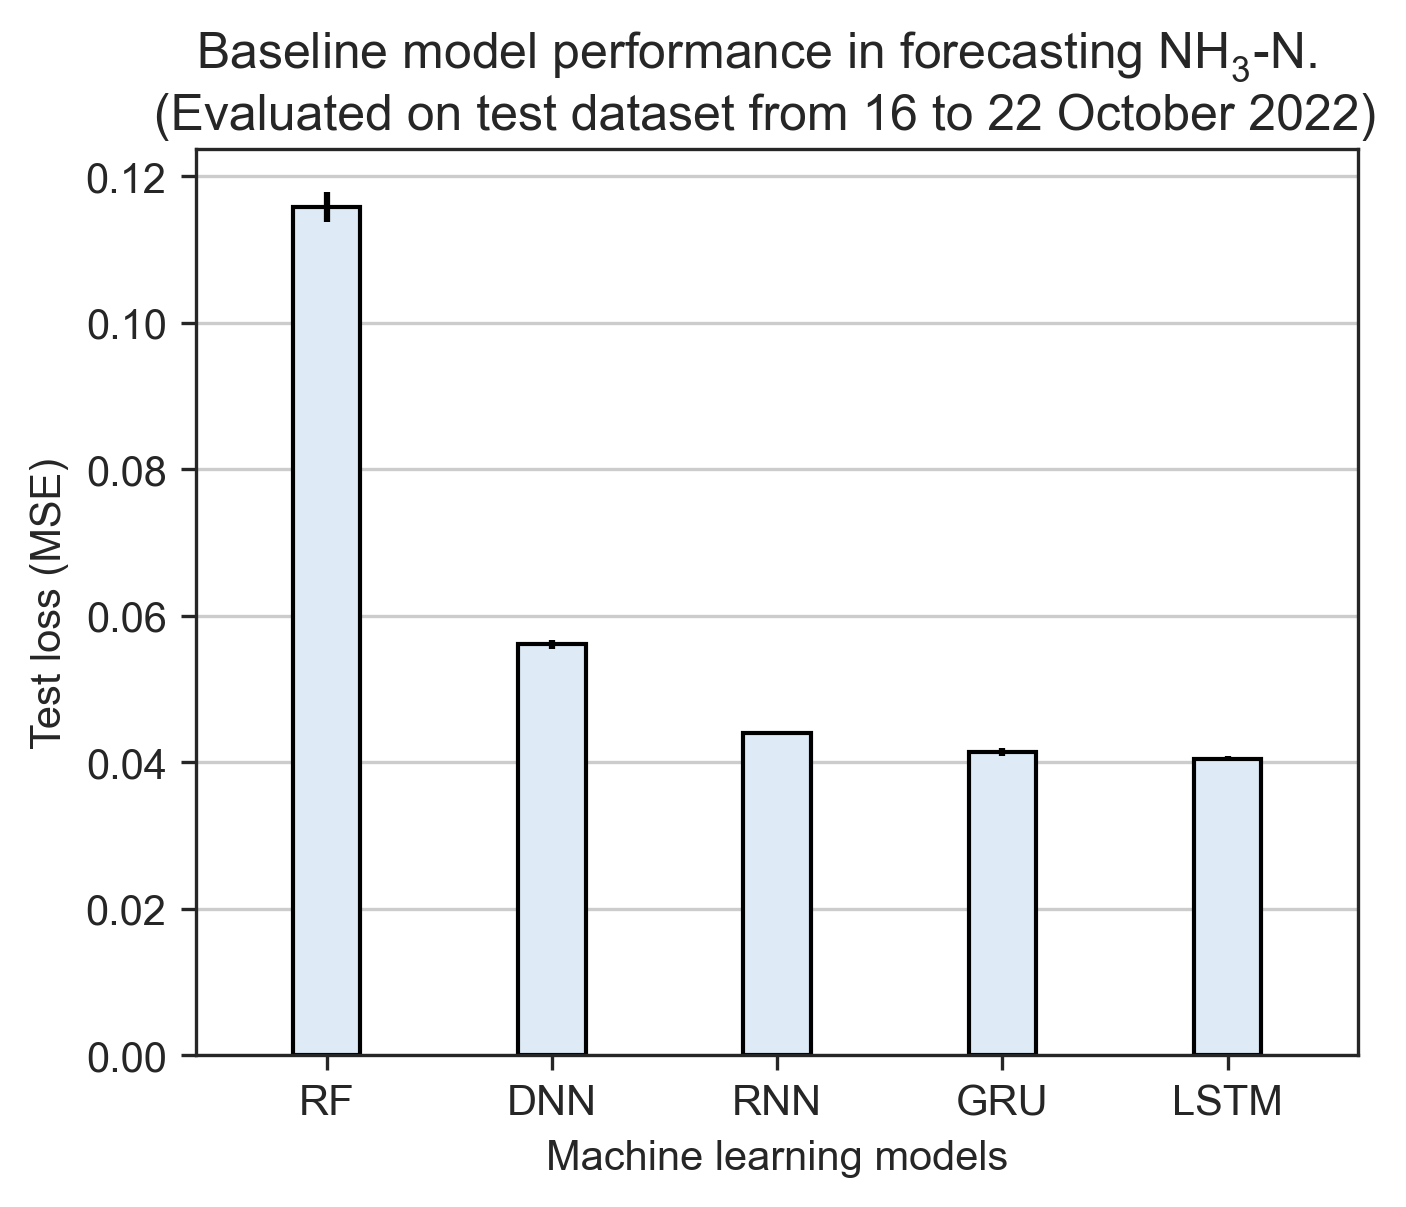
\includegraphics[width=\linewidth]{imgs/results/baseline-models-nh3.png}
      \caption{Test loss values from five ammonia forecasting models.} \label{fig:baseline-nh3}
    \end{subfigure}%
    \hspace{2em}%   % maximize separation between the subfigures
    \begin{subfigure}[t]{0.45\textwidth}
      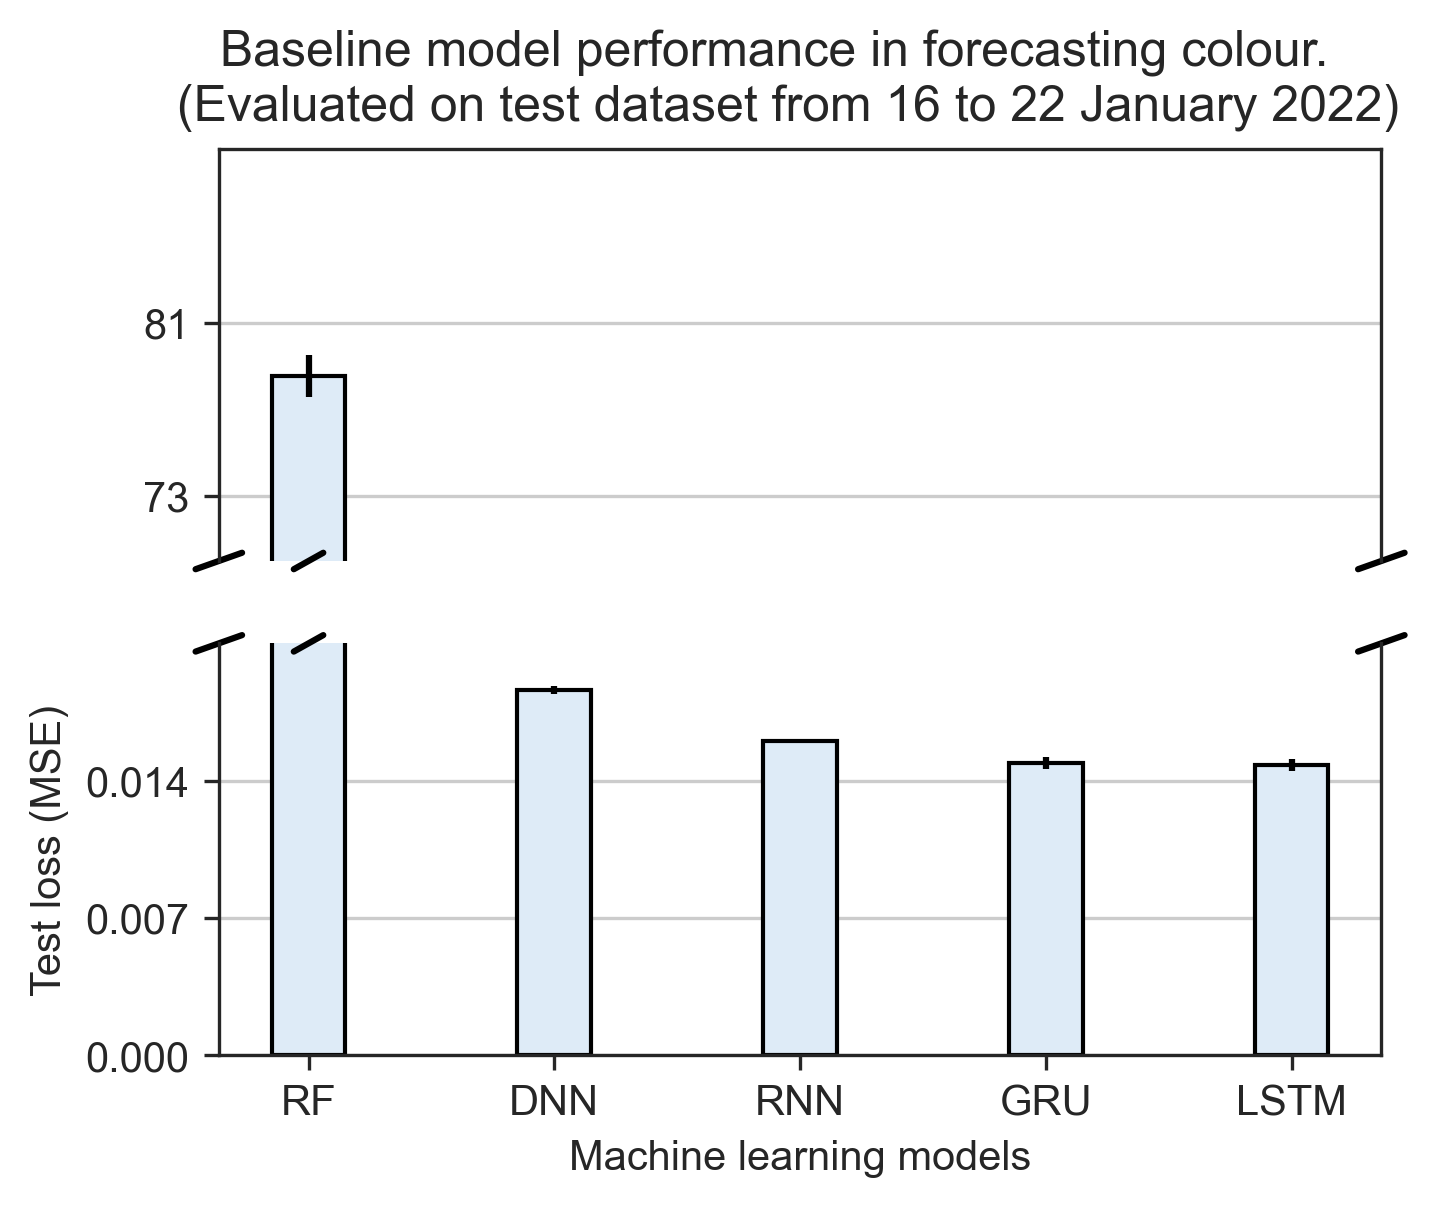
\includegraphics[width=\linewidth]{imgs/results/baseline-models-colour.png}
      \caption{Test loss values from five colour forecasting models.} \label{fig:baseline-colour}
    \end{subfigure}%  
  \caption{Baseline performance of ammonia and colour forecasting models.} \label{fig:baseline-performance}
\end{figure}

\begin{figure}[h]
    \centering
    \hspace{1em}%
    \begin{subfigure}[t]{0.45\textwidth}
      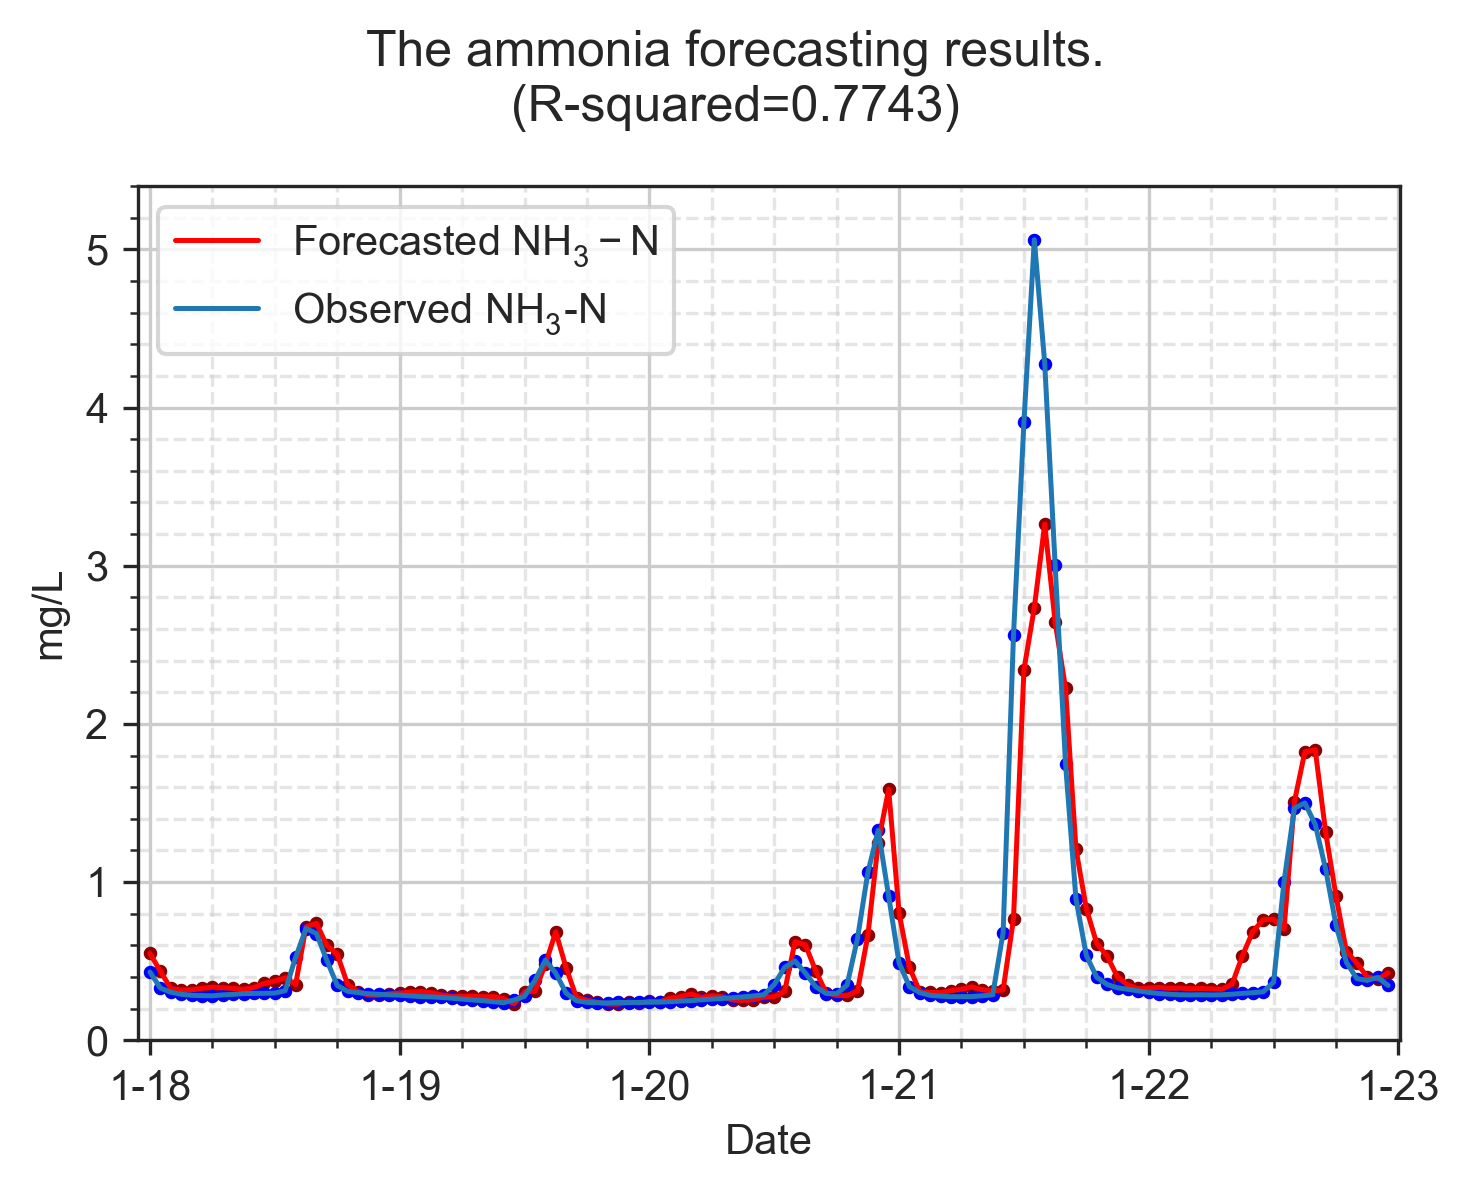
\includegraphics[width=\linewidth]{imgs/results/ammonia-colour-forecast-plot/00-RF_1_pred_Step1-obs-nh3.png}
      \caption{Baseline RF model forecasting ammonia concentration.} \label{fig:baseline-nh3-plot-rf}
    \end{subfigure}%
    \hspace{1em}%   % maximize separation between the subfigures
    \begin{subfigure}[t]{0.45\textwidth}
      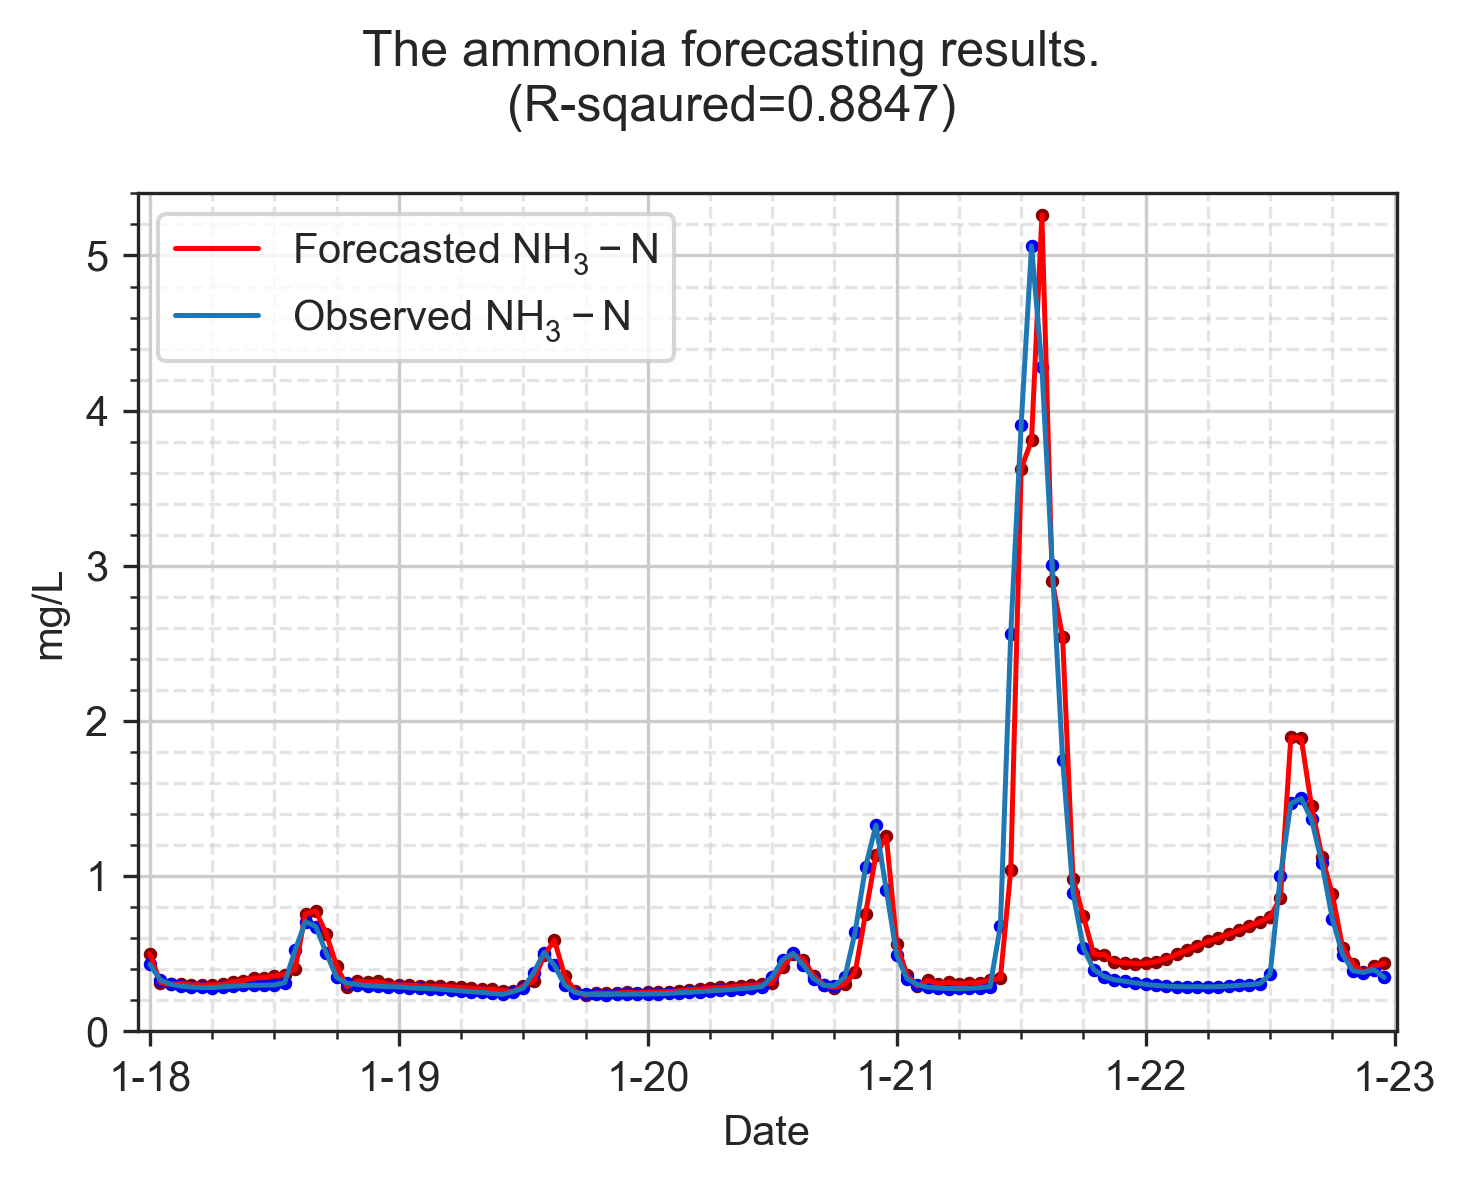
\includegraphics[width=\linewidth]{imgs/results/ammonia-colour-forecast-plot/00-LSTM_1_pred_Step1-obs-nh3.png}
      \caption{Baseline LSTM model forecasting ammonia concentration.} \label{fig:baseline-nh3-plot-lstm}
    \end{subfigure}%
    \hspace{1em}%   % maximize separation between the subfigures
    \begin{subfigure}[t]{0.45\textwidth}
      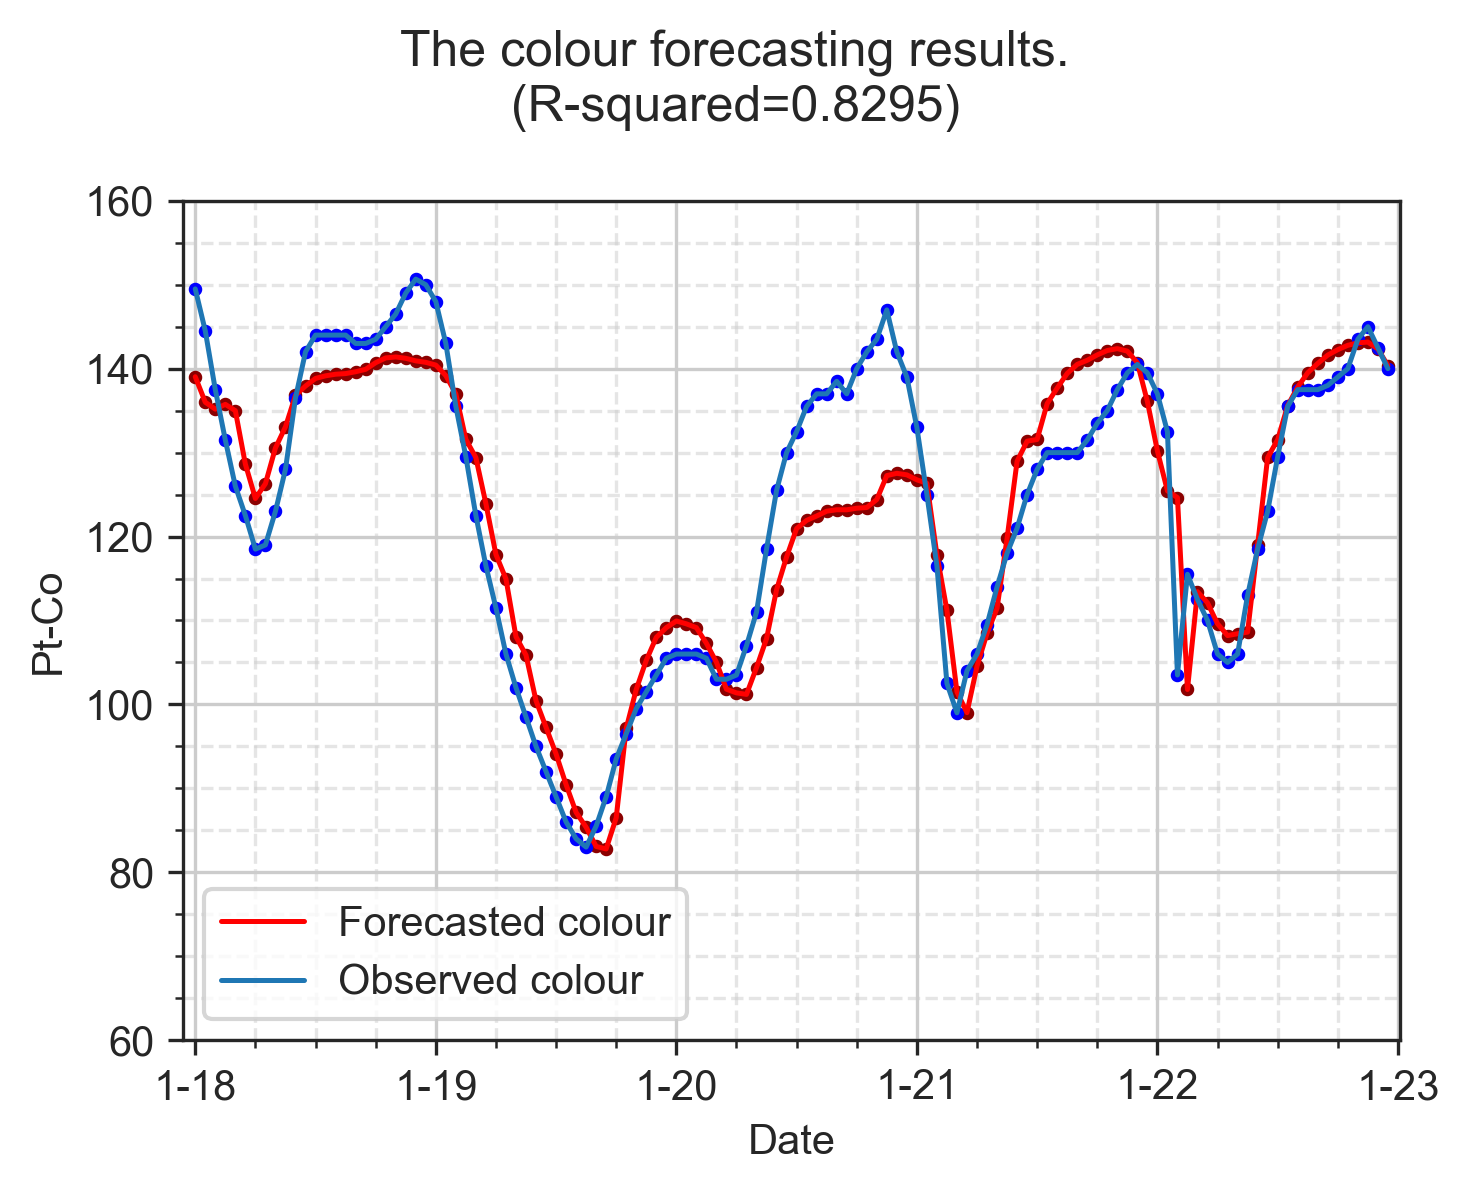
\includegraphics[width=\linewidth]{imgs/results/ammonia-colour-forecast-plot/00-RF_1_pred_Step1-obs-colour.png}
      \caption{Baseline RF model forecasting colour levels.} \label{fig:baseline-colour-plot-rf}
    \end{subfigure}% 
    \hspace{1em}%   % maximize separation between the subfigures
    \begin{subfigure}[t]{0.45\textwidth}
      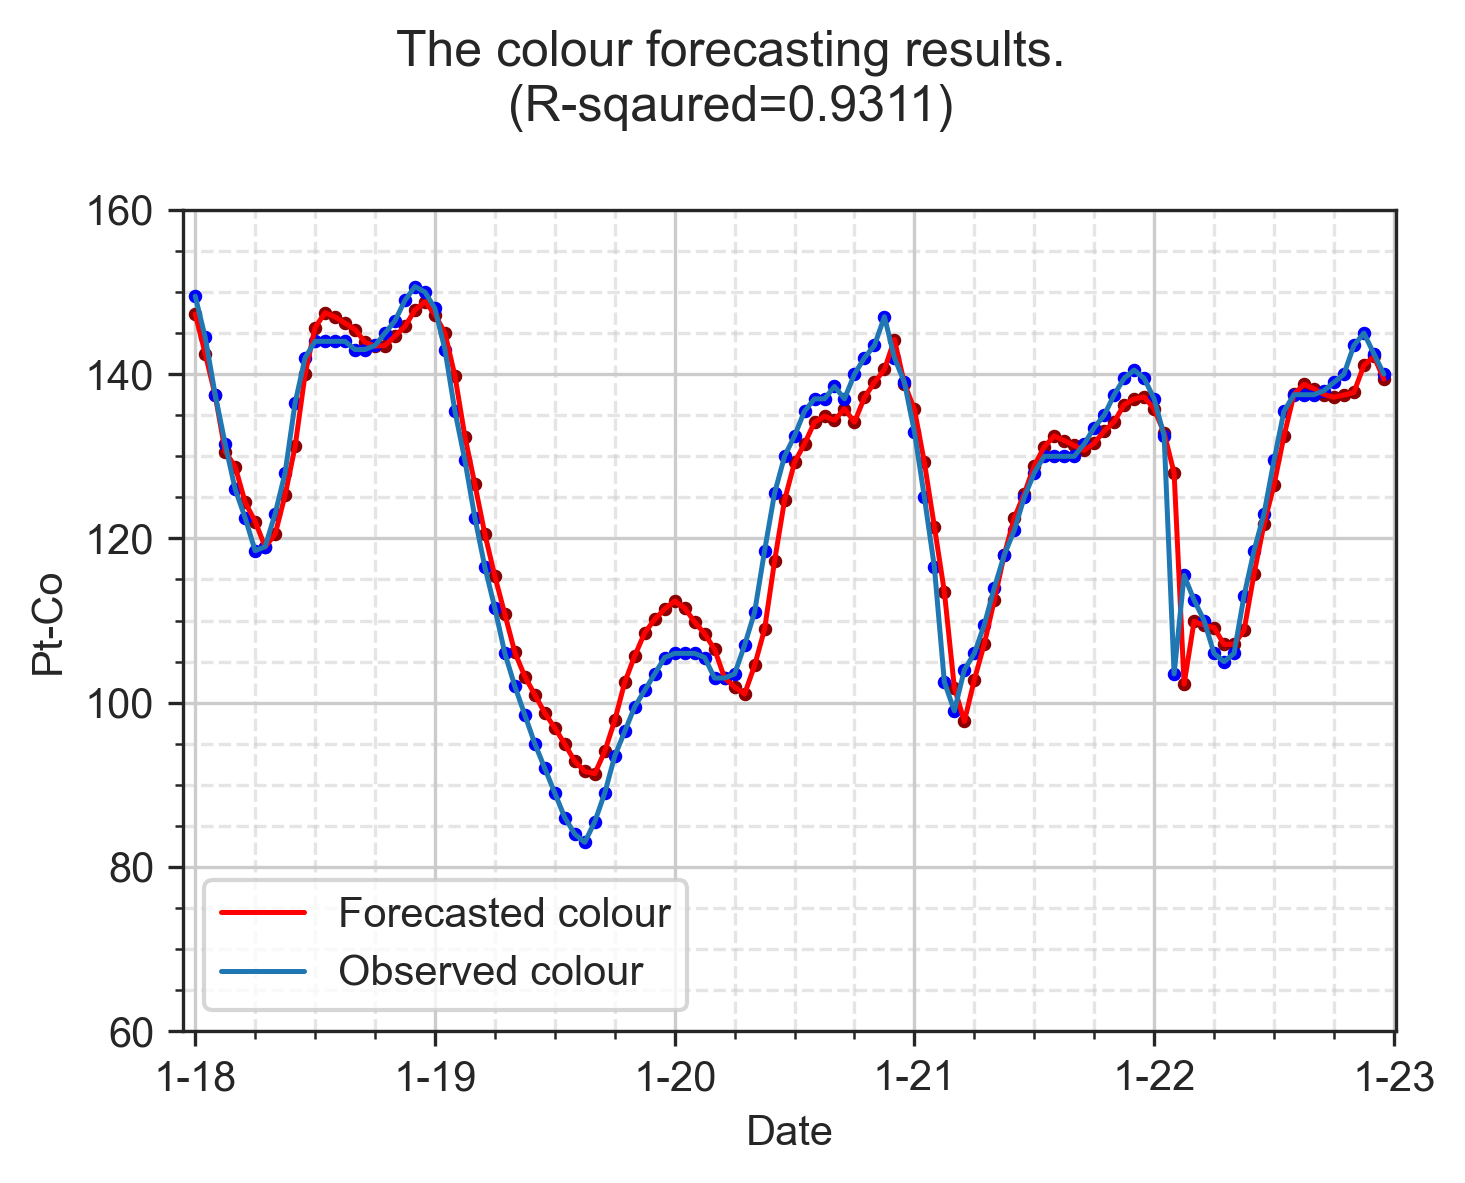
\includegraphics[width=\linewidth]{imgs/results/ammonia-colour-forecast-plot/00-LSTM_1_pred_Step1-obs-colour.png}
      \caption{Baseline LSTM model forecasting colour levels.} \label{fig:baseline-colour-plot-lstm}
    \end{subfigure}% 
  \caption{Visulization of the model forecasting results.} \label{fig:baseline-plot}
\end{figure}

\section{Improved performance on forecasting models using data pre-processing techniques}
\subsection{Models trained by pre-processed datasets}
In this study, we investigate whether the datasets treated by the proposed data pre-processing methods can improve the baseline model performance using the same hyperparameter settings. As shown in Table.~\ref{tab:baseline-result-jan-nh3} and Table.~\ref{tab:baseline-result-jan-colour}, we listed all the test loss values of five machine learning algorithms trained with each proposed pre-processed method for ammonia concentrations and colour levels forecasting. The machine learning algorithm trained by datasets that were applied with SG filters at different window sizes is denoted as model-sg5, model-sg7, and model-sg9. The naming rule applies the same to EWMA filtered dataset; the method of outlier removal for ammonia data is denoted as model-or; models trained with the raw datasets are denoted as model-obs (i.e., observed dataset).

\begin{table}[!ht]
  \centering
  \caption{Baseline performance of ammonia forecasting model, evaluated on test dataset from \textbf{16 to 22 Janurary 2022}. Loss values are calculated by MSE.}\label{tab:baseline-result-jan-nh3}
  \begin{NiceTabular}{lcclcc}
      \toprule
      Model-Dataset & Test loss & Valid loss & Model-Dataset & Test loss & Valid loss \\
      \midrule
      GRU-sg7  & 0.0383 &1.2508&RNN-or  & 0.0432&1.6345 \\
      GRU-sg5  & 0.0385 &1.2644&RNN-ew3 & 0.0434&1.6041 \\
      LSTM-ew3 & 0.0388 &1.0796&RNN-obs & 0.0440&1.6734 \\
      LSTM-sg5 & 0.0388 &1.2346&RNN-sg9 & 0.0442&1.7046 \\
      LSTM-sg7 & 0.0388 &1.1804&DNN-obs & 0.0561&3.2383 \\
      GRU-ew2  & 0.0389 &1.1891&DNN-sg5 & 0.0562&3.2170 \\
      GRU-ew4  & 0.0391 &1.2390&DNN-ew2 & 0.0563&3.1677 \\
      GRU-ew3  & 0.0392 &1.2199&DNN-ew3 & 0.0569&3.2317 \\
      LSTM-ew2 & 0.0392 &1.0969&DNN-sg7 & 0.0570&3.2014 \\
      LSTM-ew4 & 0.0395 &1.1219&DNN-ew4 & 0.0571&3.2188 \\
      GRU-sg9  & 0.0396 &1.3097&DNN-or  & 0.0572&3.1972 \\
      LSTM-or  & 0.0398 &1.2612&DNN-sg9 & 0.0574&3.2484 \\
      LSTM-obs & 0.0405 &1.3993&RF-obs  & 0.1158&- \\
      GRU-or   & 0.0405 &1.2366&RF-sg9  & 0.1196&- \\
      LSTM-sg9 & 0.0410 &1.3076&RF-ew2  & 0.1286&- \\
      GRU-obs  & 0.0414 &1.3638&RF-or   & 0.1294&- \\
      RNN-sg5  & 0.0415 &1.5088&RF-sg5  & 0.1298&- \\
      RNN-ew2  & 0.0421 &1.5425&RF-ew3  & 0.1313&- \\
      RNN-sg7  & 0.0423 &1.6267&RF-sg7  & 0.1409&- \\
      RNN-ew4  & 0.0432 &1.5992&RF-ew4  & 0.1441&- \\
      \bottomrule
  \end{NiceTabular}
\end{table}

The improvements in the performance of ammonia forecasting models are most significant with SG filters. GRU-sg5 and GRU-sg7 reduced 7.0\% and 7.4\% in the test loss compared with GRU-obs, while LSTM-sg5 and LSTM-sg7 reduced 4.2\% of the test loss compared to LSTM-obs. Both data smoothing filters reduced the test loss, and the improvements can be attributed to the modified relationships between each data point. The SG filters modified the original data points by convoluting with both previous and the following data points, which resembles the working mechanisms of recurrent neural networks, while the EWMA filter modified the data points by averaging the value of the current data point with previous ones. The performance of RF models was the poorest in the baseline model performance compared to other models. The results presented in Table.~\ref{tab:baseline-result-jan-nh3} indicate that despite RF models were trained with data pre-processing methods, the model performance in test loss was still much higher than the poorest deep learning model, which is DNN-sg9 in this case.

Empirically, when using the same testing dataset to evaluate different models, the best Model-Dataset combination should have the lowest test and validation loss values. For instance, the GRU-sg7 model in forecasting ammonia has the lowest test loss of 0.0383, yet the validation loss of 1.2508 only ranks tenth among the smallest validation loss values. The top three lowest validation loss models are LSTM-ew3, LSTM-ew2 and LSTM-ew4. This finding points to the potential of heterogeneity between the training and testing datasets. Further tests were carried out using a testing dataset from October to examine how the Model-Dataset ranks of test and validation loss values will change. To the best of my understanding, the comparisons between testing and validation loss are not discussed in the currently available research papers in the modeling of the wastewater treatment industry.

As shown in Table.~\ref{tab:baseline-result-oct-nh3}, the top three ranks of Model-Dataset in the lowest validation loss are the same as the top three ranks in the test loss values. This is in good agreement with how the heterogeneity of the datasets can impact the model performance. The evaluations of the ammonia forecasting models in October 2021 showed completely different outcomes compared to the one in January 2022. Surprisingly, the top three ranks of Model-Dataset in the lowest validation loss are the same as the lowest test loss, which are 0.0158 from LSTM-ew3, 0.0161 from LSTM-ew2, and 0.0163 from LSTM-ew4. Instead of GRU, LSTM becomes the best model for training the ammonia forecasting model. The most remarkable result in Table.~\ref{tab:baseline-result-oct-nh3} is that EWMA filter seems to be an ideal pre-processing method for training deep learning model. In the results of training different pre-processed datasets on the same machine learning algorithms, LSTM-ew3, GRU-ew3, RNN-ew4, and DNN-ew3 models showed the lowest test loss compared to the same algorithms trained by any other pre-processed datasets.

\begin{table}[!ht]
    \centering
    \caption{Baseline performance of ammonia forecasting model, evaluated on test dataset from \textbf{10 to 16 October 2021}. Loss values are calculated by MSE.}\label{tab:baseline-result-oct-nh3}
    \begin{NiceTabular}{lcclcc}
        \toprule
        Model-Dataset & Test loss & Valid loss & Model-Dataset & Test loss & Valid loss \\
        \midrule
        LSTM-ew3 & 0.0158 & 1.0796 & RNN-or  & 0.0197 & 1.6345 \\
        LSTM-ew2 & 0.0161 & 1.0969 & RNN-sg7 & 0.0201 & 1.6267 \\
        LSTM-ew4 & 0.0163 & 1.1219 & RNN-sg9 & 0.0205 & 1.7046 \\
        LSTM-sg5 & 0.0166 & 1.2346 & RNN-obs & 0.0206 & 1.6734 \\
        GRU-ew3  & 0.0167 & 1.2199 & DNN-ew3 & 0.0316 & 3.2317 \\
        GRU-ew4  & 0.0169 & 1.2390 & DNN-or  & 0.0316 & 3.1972 \\
        GRU-ew2  & 0.0170 & 1.1891 & DNN-sg7 & 0.0316 & 3.2014 \\
        GRU-sg9  & 0.0174 & 1.3097 & DNN-ew2 & 0.0318 & 3.1677 \\
        LSTM-obs & 0.0175 & 1.2366 & DNN-ew4 & 0.0319 & 3.2188 \\
        LSTM-or  & 0.0177 & 1.2612 & DNN-obs & 0.0319 & 3.2383 \\
        GRU-sg5  & 0.0178 & 1.2644 & DNN-sg5 & 0.0319 & 3.2170 \\
        GRU-sg7  & 0.0180 & 1.2508 & DNN-sg9 & 0.0319 & 3.2484 \\
        LSTM-sg7 & 0.0180 & 1.1804 & RF-sg9  & 0.1307 & - \\
        GRU-or   & 0.0187 & 1.3993 & RF-sg7  & 0.1311 & - \\
        LSTM-sg9 & 0.0188 & 1.3076 & RF-sg5  & 0.1343 & - \\
        GRU-obs  & 0.0189 & 1.3638 & RF-ew2  & 0.1346 & - \\
        RNN-ew4  & 0.0190 & 1.5992 & RF-ew3  & 0.1368 & - \\
        RNN-ew2  & 0.0191 & 1.5425 & RF-obs  & 0.1443 & - \\
        RNN-ew3  & 0.0193 & 1.6041 & RF-ew4  & 0.1451 & - \\
        RNN-sg5  & 0.0195 & 1.5088 & RF-or   & 0.1477 & - \\
        \bottomrule
    \end{NiceTabular}
\end{table}

The test loss values of the colour forecasting models are presented in Table.~\ref{tab:baseline-result-jan-colour}. The best-performed colour forecasting models are the LSTM models trained by EWMA filtered dataset, which are 0.0136 from LSTM-ew4, 0.0138 from LSTM-ew2 and LSTM-ew3. Interestingly, LSTM models trained by EWMA filtered dataset also showed the best performance in ammonia forecasting models. The top three ranks of Model-Dataset in the lowest validation loss ranks the 6th, 20th, and 1st from the lowest test loss values. However, we do not have extra testing datasets for re-evaluating the colour forecasting models. Compromises have to be made during the analysis of colour forecasting models.

\begin{table}[!ht]
  \centering
  \caption{Baseline performance of colour forecasting model, evaluated on test dataset from \textbf{16 to 22 Janurary 2022}. Loss values are calculated by MSE.}\label{tab:baseline-result-jan-colour}
  \begin{NiceTabular}{lcclcc}
      \toprule
      Model-Dataset & Test loss & Valid loss & Model-Dataset & Test loss & Valid loss \\
      \midrule
      LSTM-ew4 & 0.0136 &0.7515&RNN-obs  & 0.0160 &1.0623 \\
      LSTM-ew2 & 0.0138 &0.8011&LSTM-sg7 & 0.0161 &0.7439 \\
      LSTM-ew3 & 0.0138 &0.7547&LSTM-sg5 & 0.0168 &0.8355 \\
      GRU-ew3  & 0.0140 &0.8068&DNN-sg5  & 0.0180 &1.4702 \\
      GRU-ew2  & 0.0142 &0.8330&DNN-sg7  & 0.0180 &1.4823 \\
      GRU-ew4  & 0.0143 &0.7694&DNN-sg9  & 0.0180 &1.4574 \\
      LSTM-sg9 & 0.0143 &0.7137&DNN-ew4  & 0.0181 &1.4632 \\
      RNN-ew3  & 0.0144 &0.8492&DNN-ew3  & 0.0182 &1.4716 \\
      RNN-ew4  & 0.0147 &0.8476&DNN-ew2  & 0.0183 &1.4946 \\
      RNN-sg9  & 0.0147 &0.8363&DNN-obs  & 0.0186 &1.5397 \\
      LSTM-obs & 0.0148 &0.9744&RF-sg9   & 63.6847& \\
      GRU-obs  & 0.0149 &0.9927&RF-sg7   & 73.8263& \\
      RNN-ew2  & 0.0150 &0.9083&RF-ew3   & 75.1974&- \\
      GRU-sg9  & 0.0151 &0.7575&RF-ew4   & 77.8829&- \\
      RNN-sg5  & 0.0158 &0.8846&RF-obs   & 78.5296&- \\
      RNN-sg7  & 0.0158 &0.8755&RF-ew2   & 78.8753&- \\
      GRU-sg7  & 0.0159 &0.7791&RF-sg5   & 81.0696&- \\
      GRU-sg5  & 0.0160 &0.8080&    -    &     -  &- \\
      \bottomrule
  \end{NiceTabular}
\end{table}

By comparing the baseline performance and the influences of data pre-processing techniques on machine learning models, our findings appear to be well substantiated by the use of LSTM models for training ammonia and colour forecasting models due to their outstanding model performance evaluated by test loss values. Although EWMA filters showed surprising effects on improving the performance of most models, the influence of pre-processing methods is still not consistent across different models and training datasets. Thus, the testings of the proposed model training processes will include all the pre-processing techniques for model training, and LSTM will be used as the only machine learning model.

\subsection{The effect of window size of data smoothing filters}

\begin{figure}[h]
  \centering
  \begin{subfigure}[t]{0.45\textwidth}
    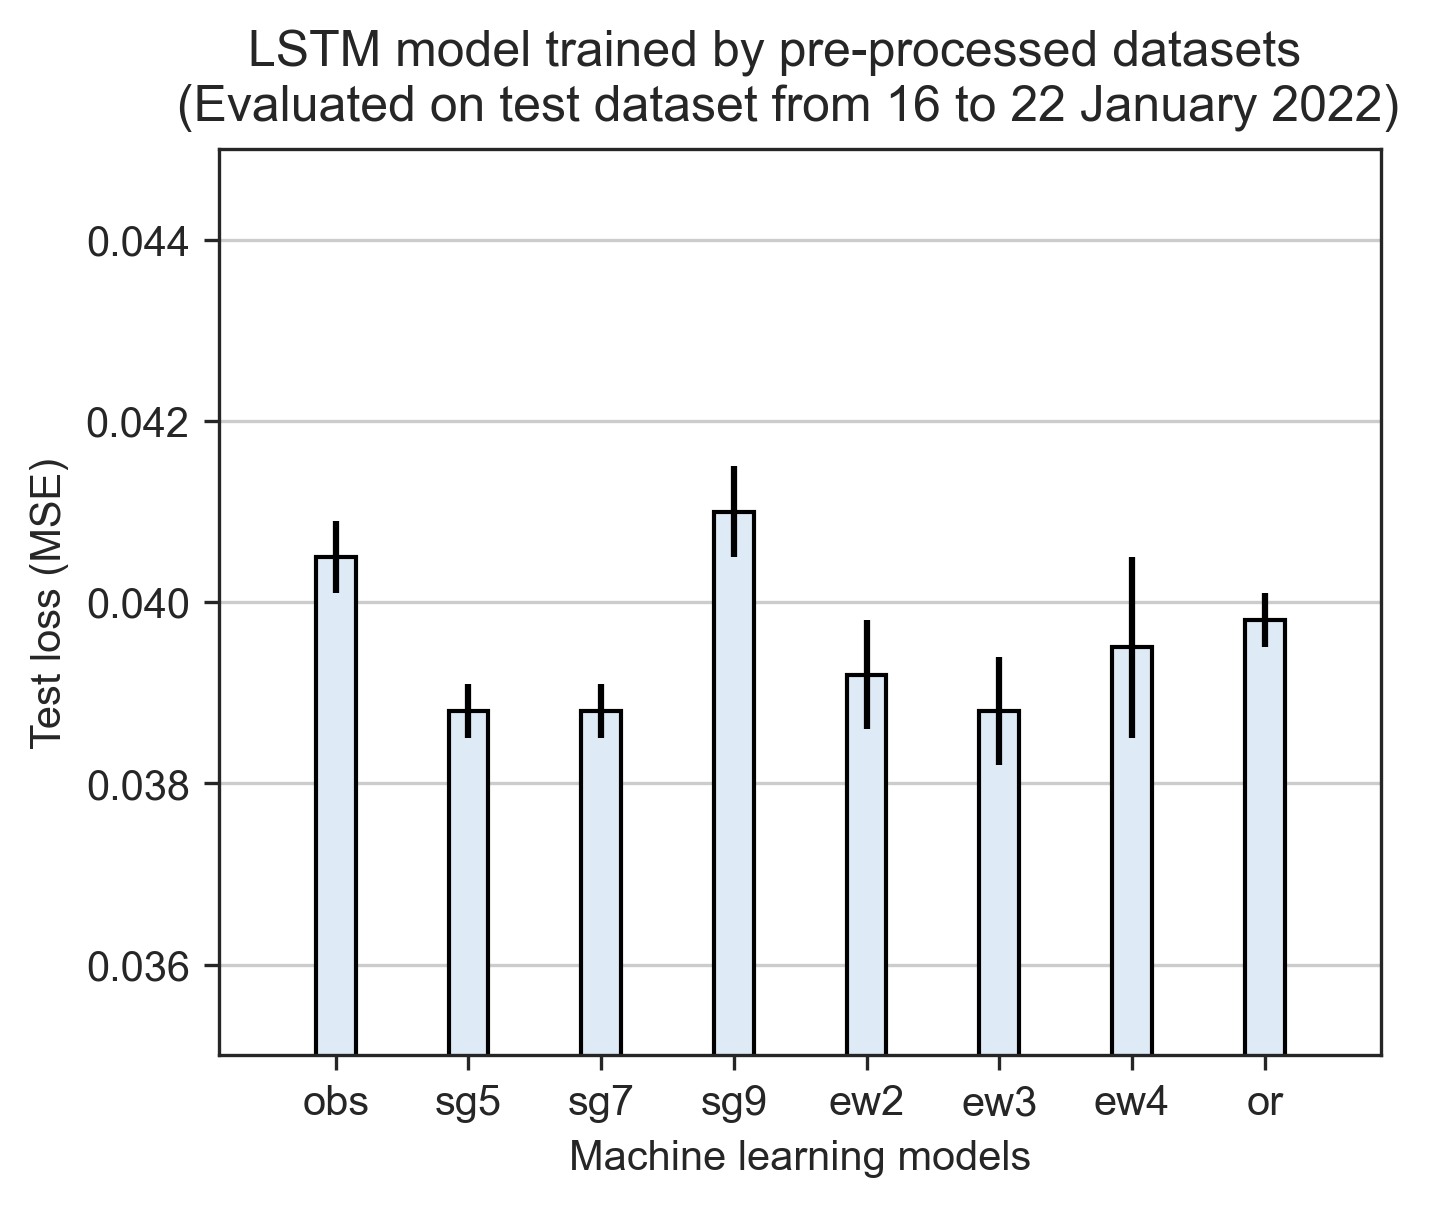
\includegraphics[width=\linewidth]{imgs/results/feature-engineering/pre-processing-nh3-jan.png}
    \caption{Baseline performance of ammonia forecasting models trained by LSTM.} \label{fig:preprocessing-nh3}
  \end{subfigure}
  \hspace{2em}
  \begin{subfigure}[t]{0.45\textwidth}
    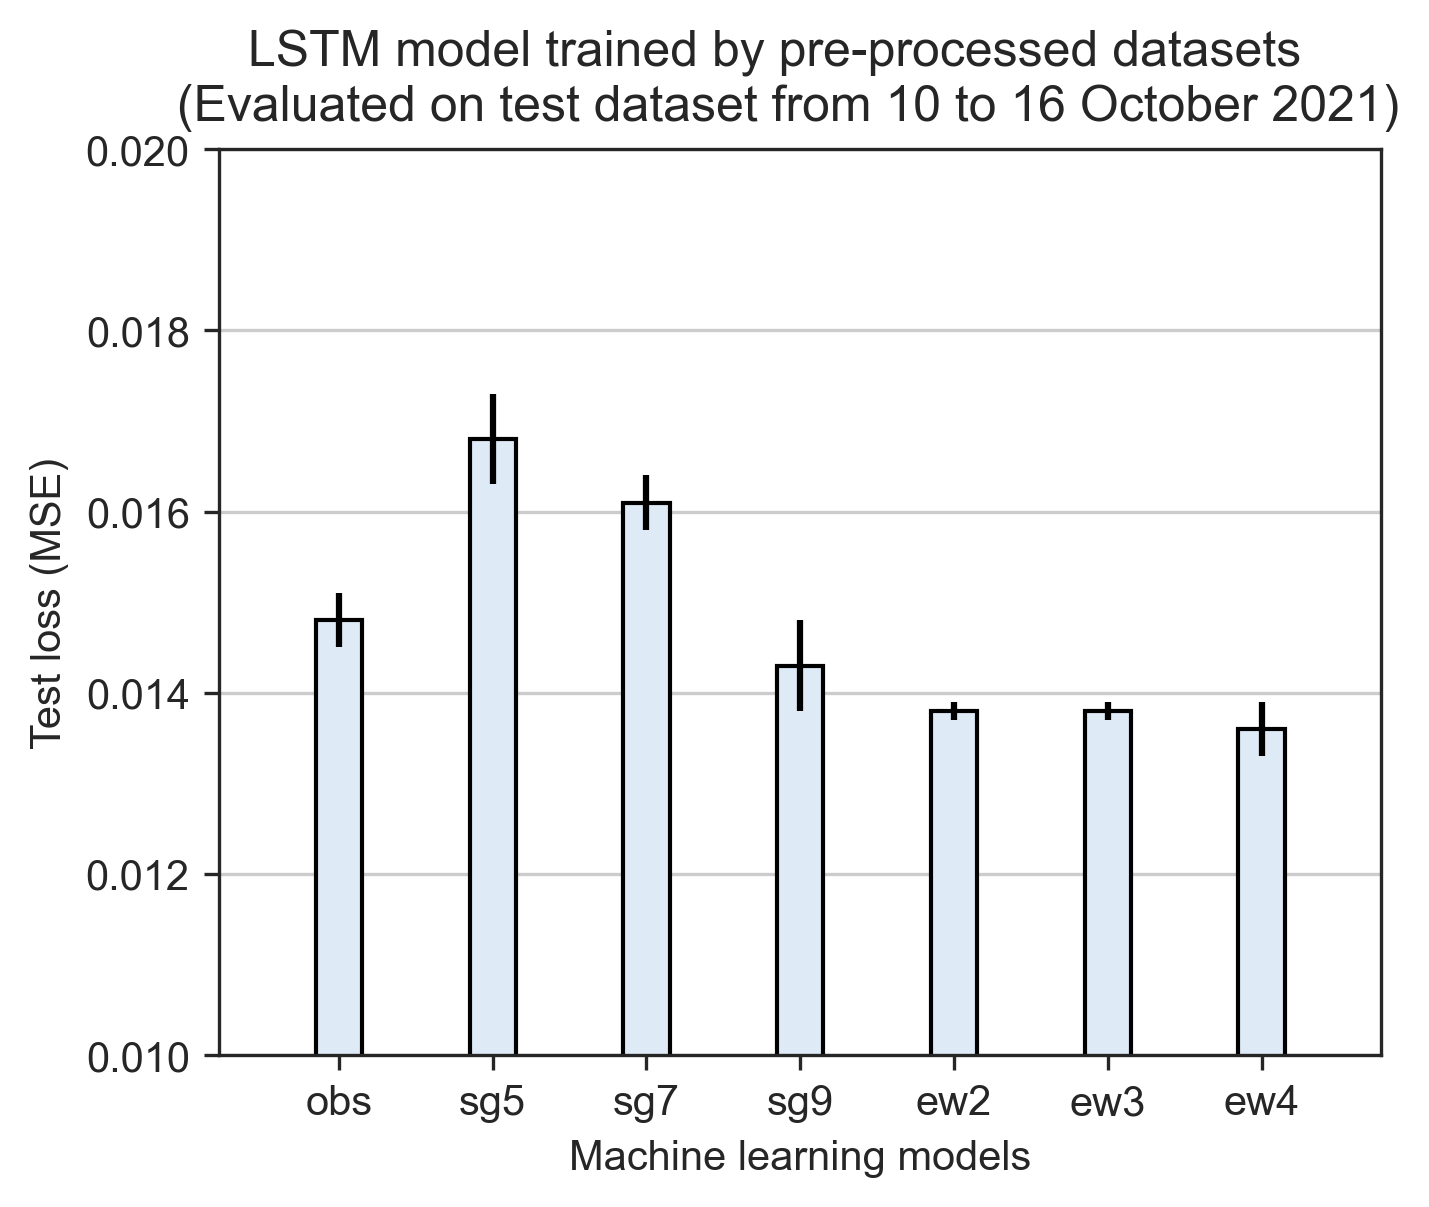
\includegraphics[width=\linewidth]{imgs/results/feature-engineering/pre-processing-colour.png}
    \caption{Baseline performance of colour forecasting models trained by LSTM.} \label{fig:preprocessing-colour}
  \end{subfigure}
\caption{Baseline performance of ammonia and colour forecasting models.} \label{fig:preprocessing-comparison}
\end{figure}
The influences of window sizes in the data smoothing process are investigated using LSTM models and illustrated in Fig.~\ref{fig:preprocessing-comparison}. SG window sizes of higher and lower have different impacts on ammonia and colour forecasting models. For instance, LSTM-sg5 performed better than LSTM-sg9 in forecasting ammonia, and LSTM-sg9 outperformed LSTM-sg5 in forecasting colour. A similar pattern can also be observed in models trained by EWMA filters. For the ammonia forecasting model, LSTM-ew3 is better, while for the colour forecasting model, LSTM-ew4 is better. Therefore, the data smoothing filters' window sizes must be carefully selected. The unpredictable influences of applying data smoothing filters on forecasting models impede the determination of the optimal data smoothing method in the subsequent experiments. All the pre-processing techniques will be applied to the LSTM models for further studies.

\section{Exploit hidden patterns in MBR effluent water quality to enhance model performance}
\subsection{Ammonia forecasting models}
In the section of feature engineering, we have introduced the selection and creation of the extra input features for training forecasting models, as shown in Fig.~\ref{fig:feature-selection}. In this study, a forecasting model trained by one feature is called an univariate model and denoted as LSTM-1; a forecasting model trained by two features is called a multivariate model and denoted as LSTM-2. For models trained by three and four features are denoted as LSTM-3 and LSTM-4. In Fig.~\ref{fig:nh3-feature-engineering}, the performance of ammonia forecasting models trained by two to four inputs (i.e., LSTM-2, LSTM-3, LSTM-4) is compared with the baseline performance (i.e., LSTM-1-obs) to demonstrate how the feature engineered features influenced on the model outputs. 
%Notice that due to colour data are not available from 10 to 16 October 2021, the models in Fig.~\ref{fig:colour-feature-engineering} were evaluated on training dataset from 16 to 22 January 2022. 

As shown in Fig.~\ref{fig:nh3-feature-engineering}, LSTM-4-obs showed the highest test loss, followed by LSTM-3-obs, LSTM-2-obs and LSTM-1-obs. This result indicates that LSTM models trained with more features can result in poorer model performance. Based on our understanding to the extra features such as color levels and sine/cosine features, models trained with more features are expected lower test values. The model performance from LSTM-sg7 and LSTM-sg9 fits well with what we hypothesized. The results showed that the test loss values of the LSTM models trained by sg7 and sg9 filtered datasets followed the trend of LSTM-4$<$LSTM-3$<$LSTM-2$<$LSTM-1. The most remarkable results are from LSTM models trained by SG filtered dataset at a window size of 7. Comparing to the baseline model performance (i.e., LSTM-1-obs), the test loss values of LSTM-1-sg7, LSTM-2-sg7, LSTM-3-sg7 and LSTM-4-sg7 reduced by 4.2\%, 6.4\%, 7.9\%, and 8.9\%, respectively. 

Our findings in the ammonia forecasting models suggest that colour level is an indispensable input for improving the model performance. LSTM-2 models trained by datasets applied with any pre-processing techniques showed lower test loss compared to LSTM-1, except LSTM-2 trained by dataset without applying any methods. Strong evidence leads us to believe that the fluctuation of ammonia concentration is highly correlated with the colour level in SHWEPP influent even without direct evidence.

The methods of training LSTM models on pre-processed datasets have proved their benefits in improving baseline model performance. Yet, the test loss values were only reduced slightly for those models trained with EWMA filtered datasets. As shown in Fig.~\ref{fig:nh3-feature-engineering}, LSTM-3-ew2, LSTM-4-ew2, LSTM-3-ew4, and LSTM-4-ew4 shared very similar test loss values to LSTM-1-obs, indicating the advantages of enhanced quality in training dataset were not fully reflected on the model performance when LSTM models were trained by EWMA filtered datasets.

\begin{figure}[h]
    \centering
    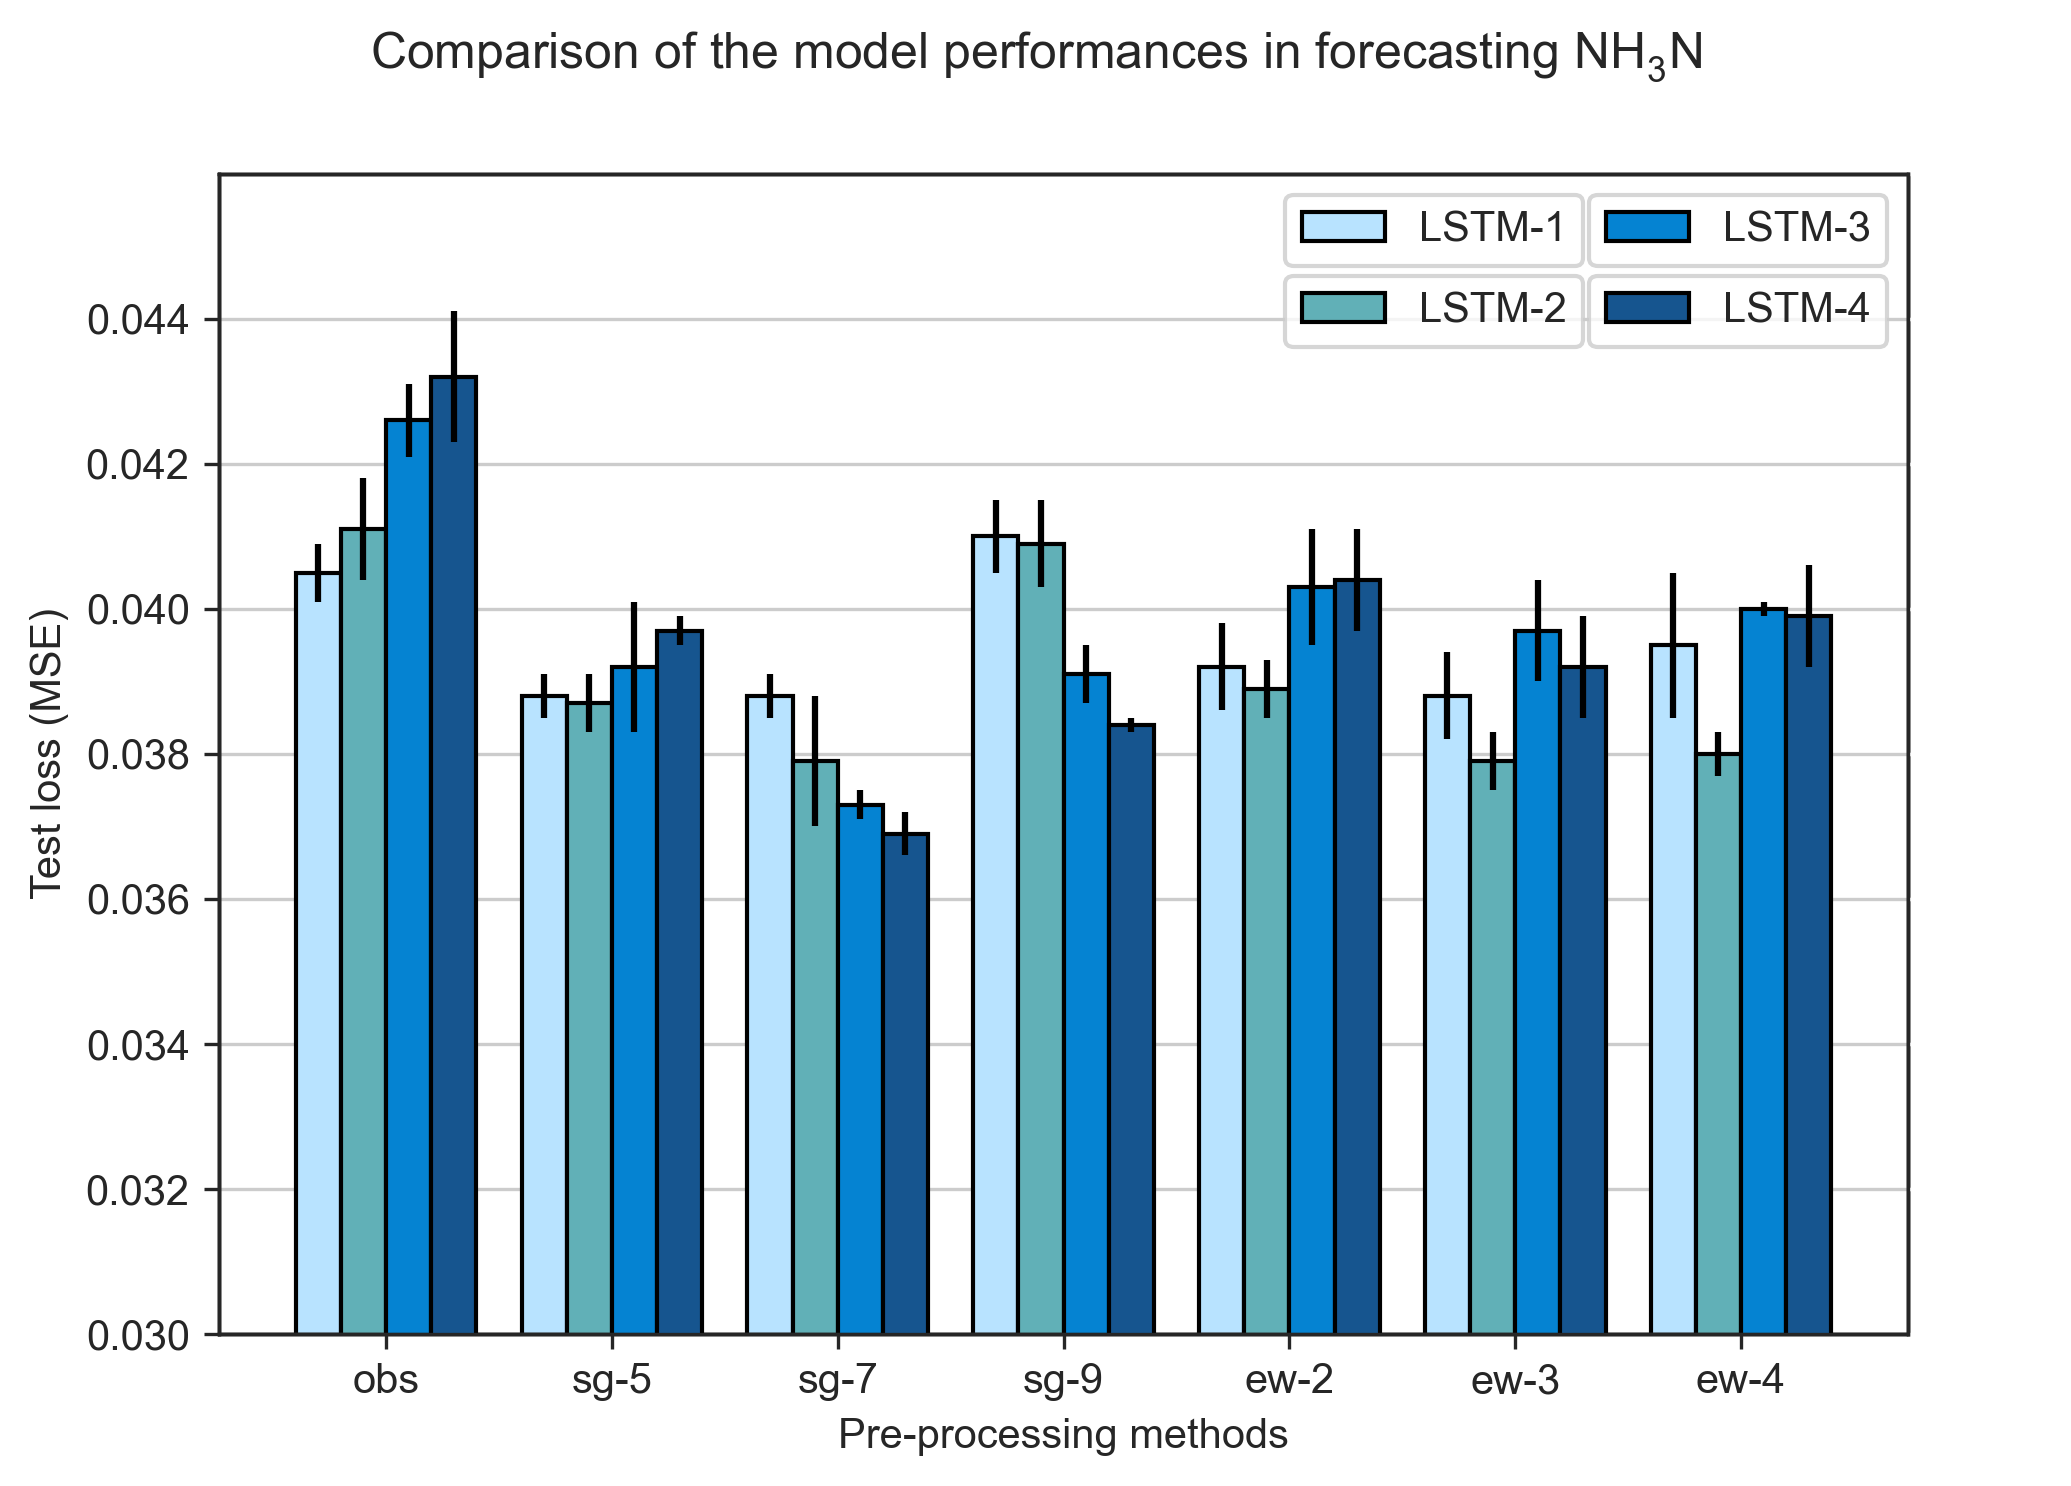
\includegraphics[width=0.6\columnwidth]{imgs/results/feature-engineering/nh3-input-1-4-comparison.png}
    \caption{Comparisons of the model performance in forecasitng ammonia concentrations.}
    \label{fig:nh3-feature-engineering}
 \end{figure}

\subsection{Colour forecasting models}

As shown in Fig.~\ref{fig:colour-feature-engineering}, most of the proposed pre-processing techniques improved the performance of colour forecasting models. All the LSTM models trained by EWMA filtered datasets have lower test loss compared to the baseline model performance, while part of the LSTM models trained by SG filtered datasets showed improvement in the model performance. The performance of models trained by SG filtered datasets was rather disappointing. We observed that the test loss of LSTM-sg5, LSTM-sg7, and LSTM-sg9 showed much higher values of standard deviations, and this was probably due to the poor quality of the raw colour data. 

From the results of ammonia forecasting models, we thought that LSTM models trained by sg7 filtered dataset would generate the lowest test loss in LSTM-4. However, the results in the colour forecasting models revealed that the lowest test loss was generated from LSTM-3-sg9, with test values of 0.0121, a 28.6\% improvement in model performance compared to the baseline model performance. Contrary to expectations, datasets trained by four inputs failed to generate the lowest test loss. The fact of having higher test loss in LSTM-4 compared to LSTM-3 is evident and can be found in Fig.~\ref{fig:colour-feature-engineering} except LSTM-4-sg7. It is very likely that including ammonia concentrations as an input feature worsened the quality of the training dataset and resulted in poorer performance for colour forecasting models.


%\noindent
%\begin{myenumerate}
%    \item In the results of LSTM-sg7, the test values decreased with the increased number of model inputs, which satified the hypothesis we claimed in previous section.
%    \item The test loss values of LSTM-2 in all the pre-processed datasets are lower than LSTM-1 except for LSTM-obs, LSTM-sg9 and LSTM-ew2.
%    \item In LSTM-obs, models trained with more inputs resulted in poorer model performance, except for LSTM-obs, LSTM-sg9 and LSTM-ew2.
%\end{myenumerate}


\begin{figure}[t]
    \centering
    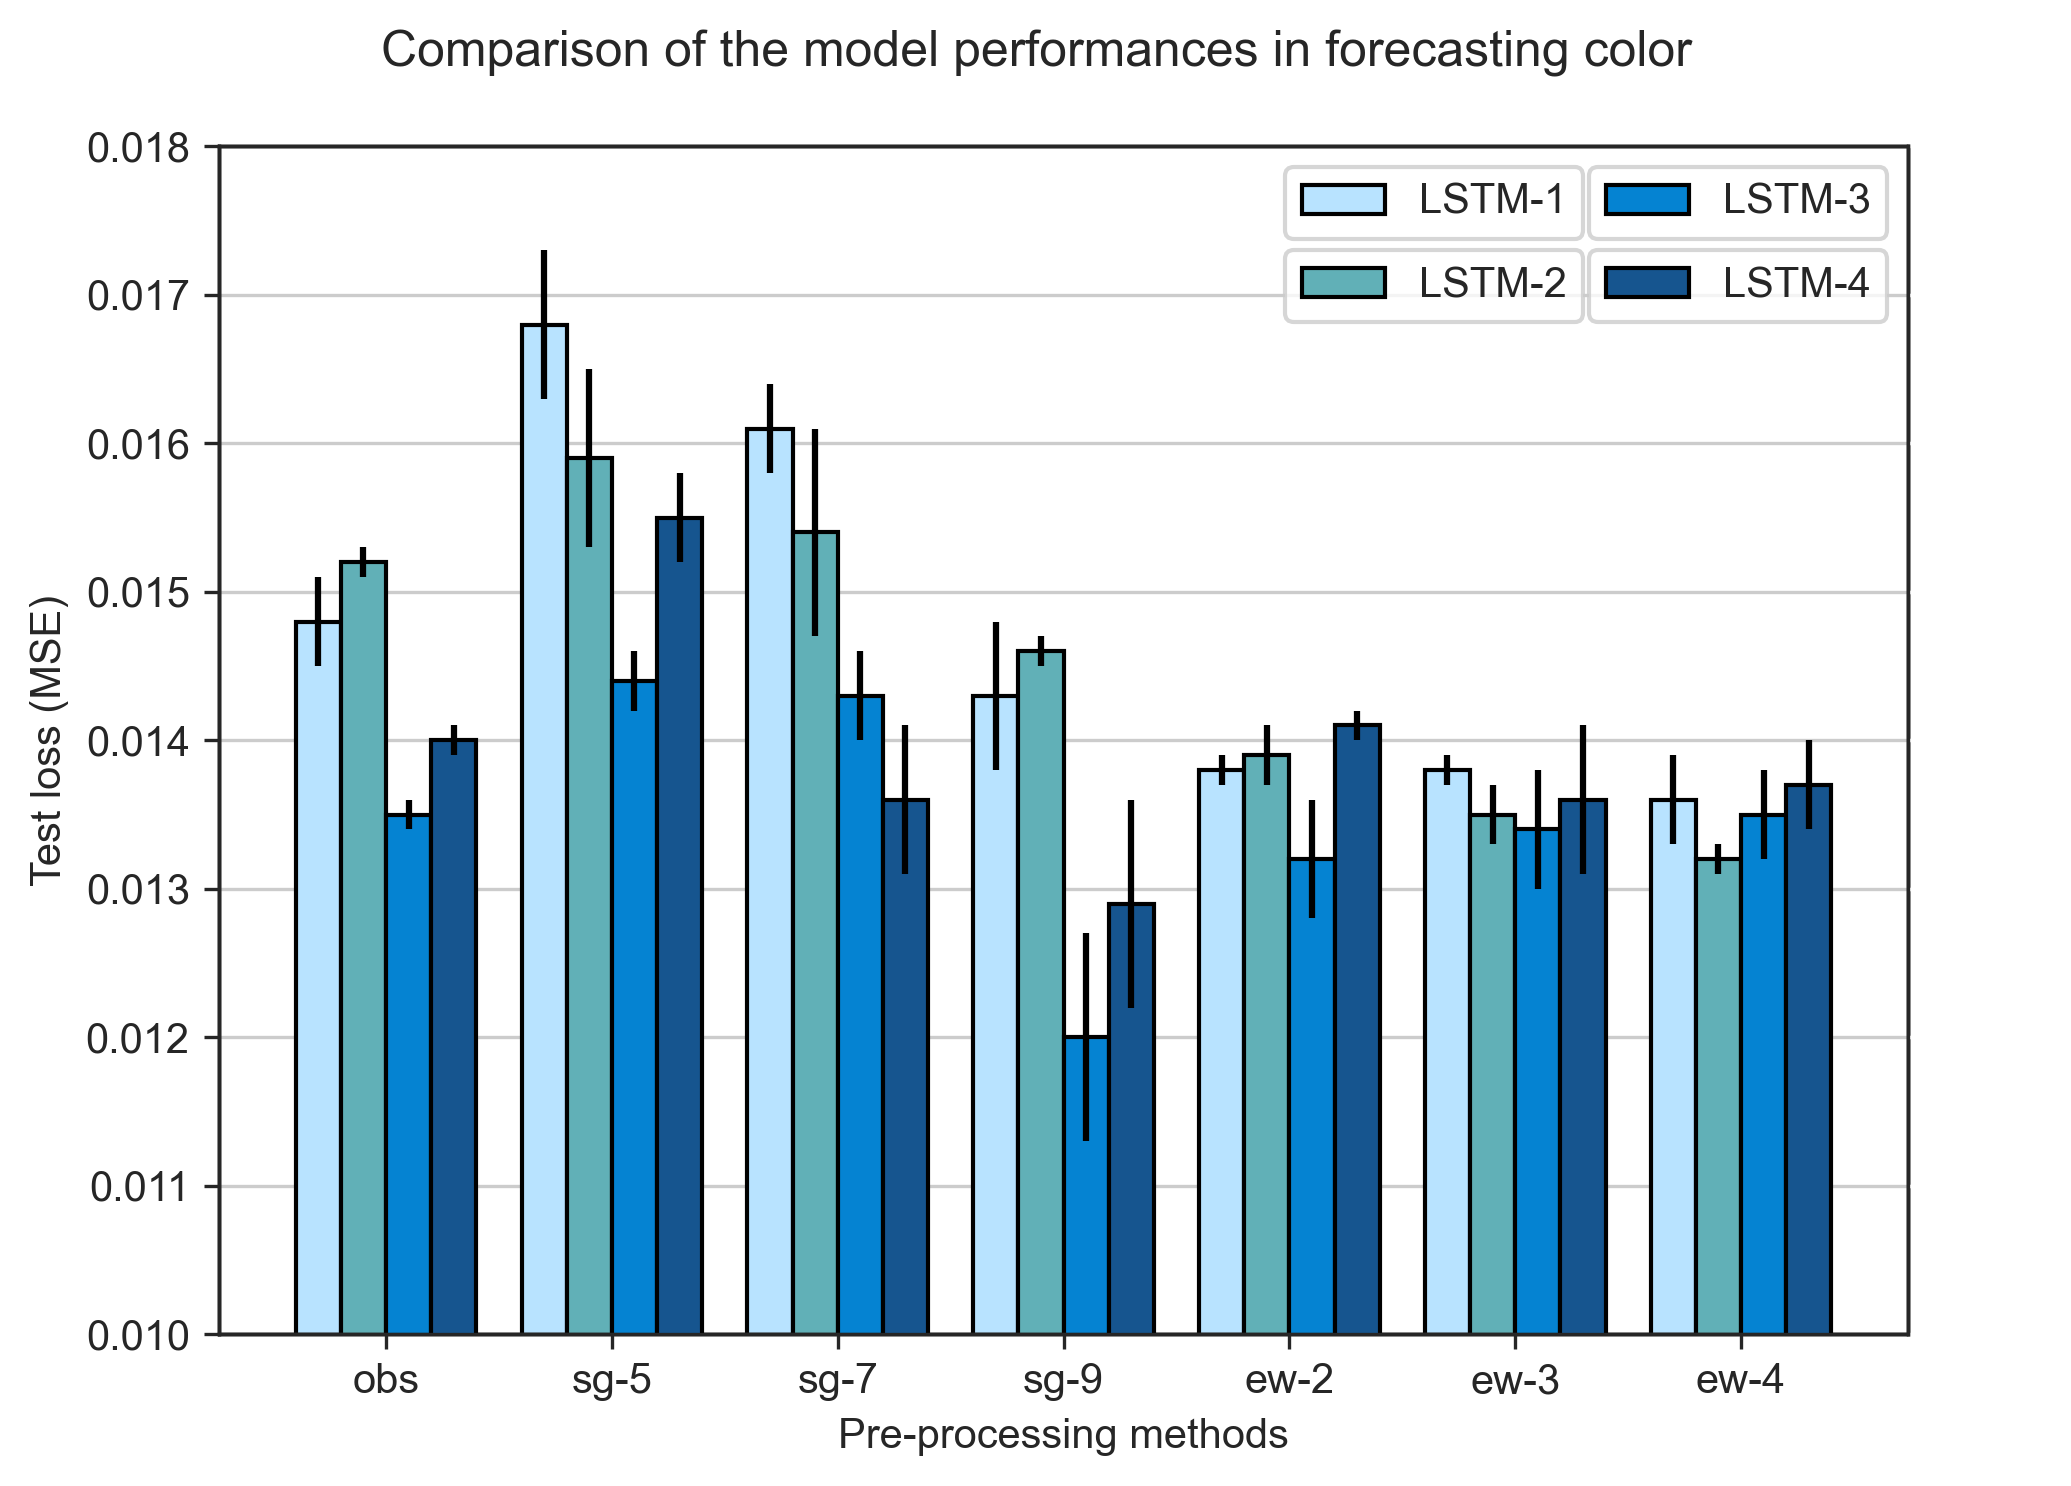
\includegraphics[width=0.6\columnwidth]{imgs/results/feature-engineering/colour-input-1-4-comparison.png}
    \caption{Comparisons of model performance in forecasting colour levels.}
    \label{fig:colour-feature-engineering}
 \end{figure}

%\section{Design of model architecture through analyzing wastewater composition in sewer system}

\chapter{Conclusions and Recommendation}
\section{Conclusions}
\subsection{Machine learning models vs deep learning models}
The selection of using which machine learning and deep learning models was not widely discussed to the best of our knowledge in the modelling of wastewater treatment industry. This study has investigated on the model performance of machine learning model of RF, and four other deep learning models of DNN, RNN, GRU and LSTM on forecasting ammonia concentrations and colour levels in reclaimed water system for assisting treatment operation and management. The evidence from this study suggests deep learning models are much capable in learning from the historical data and generate more accurate forecasting results. In both ammonia and colour forecasting models, the test loss values of RF are much higher than the values from the least performanced deep learning model of DNN. Among all the deep learning models, the results indicate LSTM and GRU models have the lowest test loss of 0.0405 and 0.0414, respectively. However, the further research works suggest LSTM models trained with pre-processing methods generate the lowest test loss compared to GRU, making the LSTM model the most promising recurrent neural network model for training forecasting models.

\subsection{Data pre-processing methods}
Our research also highlighted the importance of how the model performance can be improved from applying data pre-processing and feature engineering techniques. Generally speaking, all the proposed data smoothing and outlier removal methods reduced the test loss values compared to the baseline model performance (i.e., the window sizes of the filters need to be carefully selected), as showin in Fig.~\ref{fig:preprocessing-comparison}.

%This paper has investigated on how much the data pre-processed methods and feature engineering techniques can improve the performance on the ammonia and colour forecasting models. The evidence from this study suggests ammonia forecasting model trained by SG filter (i.e., LSTM-1-sg7) reduced test loss by 4.2\%, and model trained with engineered features (i.e., LSTM-4-sg7) reduced test loss by 8.9\%. Showing 

\subsection{Feature engineering}
This study is the first step towards enhancing our understanding to the potential benefits of using created features for model training. The thorough examinations of the Geomap nearby the SHWEPP and the investigation of water composition in the public sewege system helped us to hypothesize that the change of ammonia concentrations and colour levels are dependent to each other. With the help of additional colour/ammonia data for ammonia/colour forecasting model, the test loss reduced by 6.4\% (i.e., LSTM-2-sg7 compared to LSTM-1-obs) and 10.8\% (i.e., LSTM-2-ew4 compared to LSTM-1-obs), respectively. 

Moreover, the similarity between the household consumption patterns and the daily fluctuation of ammonia concentrations have unexpectedly helped us to formulate the time features via positional encoding. The influence of the sine and cosine hour features on the model perfromance showed tremendous improvements on both ammonia and colour forecasting models. In the former, test loss dropped by 8.9\% (i.e., LSTM-1-obs compared with LSTM-4-sg7) while the latter reduced by 28.6\% (i.e., LSTM-1-obs compared with LSTM-3-sg9). The remarkable use of positional encoding features is it is not limited to just ammonia and colour forecasting models. Any time series data characterized with daily fluctuation patterns can adopt the use of the features of sine and cosine hour as long as the patterns are based on actaul events. In addition, the positional encoding features are not limited to hour, we can encode features into from seconds to weeks, and even years, the application of it is infinite. However, the feature engineering method clearly has some limitations. In the results of ammonia forecasting models, LSTM-2-obs, LSTM-3-obs and LSTM-4-obs showed higher tess loss compared to LSTM-1-obs, indicating when the models were trained by any features other than ammonia, the model performance worsened. In addition to that, when extra features were train with EWMA filters, the test loss increased, and the worsening of model performance also occured on colour forecasting models trained by EWMA filters. Our results suggest that feature engineering needs to be carefully evaluated and experimented before the real use. Despite the limitations, the combination use of feature engineering in building ammonia and colour forecasting models in this study has fully proved it's advantages. 

\section{Recommendations for future research}
Due to the insufficient ammonia and colour data, we cannot differentiate whether the undesired model performance was caused by the heterogeneity of the training and testing datasets or caused by the pre-processing and feature engineering methods we applied on the datasets. It is recommended a larger dataset (e.g., dataset with the size of 2 months or longer) should be used in the future study when evaluating the proposed methods in this study. The insufficient amount of data could also lead to the unstable performance of different models trained by the same data smoothing methods. For instance, LSTM-4-sg7 and LSTM-3-sg7 have the lowest test loss among LSTM-4 and LSTM-3 models, however, LSTM-2-ew4 has the lower test loss than LSTM-4-sg7. We failed to explain what has caused such outcome. 

All the forecasting models in this study only focus on predicting ammonia concentration and colour levles, and in the futher study, more water quality parameters should be included. In reclaimed water system, the concentration of water quality parameters such as turbidity and E. coli are also regulated by Water Supply Department. The violation of any water quality parameter will directly lead to the disqualification of being used as reclaimed water. Moreover, The hidden correlations reside between each water quality parameter will most likely be helpful in building any water quality forecasting models.

?????

% \showthe\font
%%%%%%%%%%%%%%%%%%%%%%%%%%%%%%%%%%%%%%%%%%%%%%%%%%%%%%%%%%%%%%%%%%%%%%%%%
%                                                                       %
%      9) BIBLIOGRAPHY                                                  %
%                                                                       %
% This example uses bibtex to generate the required Bibliography. Refer %
% to the % the file ustthesis_test.bib for the entries of the           %
% Bibliography. Note that only the cited entries are printed.           %
%                                                                       %
% If BibTeX is not used to typeset the bibliography, replace the        %
% following line with the \begin{thebibliography} and \end{bibliography}%
% commands (the "thebibliography" environment) to process the           %
% Bibliography.                                                         %
%                                                                       %
%%%%%%%%%%%%%%%%%%%%%%%%%%%%%%%%%%%%%%%%%%%%%%%%%%%%%%%%%%%%%%%%%%%%%%%%%

%%%%%%%%%%%%%%%%%%%%%%%%%%%%%%%%%%%%%%%%%%%%%%%%%%%%%%%%%%%%%%%%%%%%%%%%%
%                                                                       %
% The recommended bibliography style is the IEEE bibliography style.    %
% "ustbib" defines the IEEE bibliography standard with the added        %
% ability of sorting the items by name of author.                       %
%                                                                       %
% If you are not using BibTeX to process your Bibliography, comment out %
% the following line.                                                   %
%                                                                       %
%%%%%%%%%%%%%%%%%%%%%%%%%%%%%%%%%%%%%%%%%%%%%%%%%%%%%%%%%%%%%%%%%%%%%%%%%
%\addcontentsline{toc}{section}{References}
\bibliographystyle{plainnat}

\bibliography{MPhil-thesis-papers}

%%%%%%%%%%%%%%%%%%%%%%%%%%%%%%%%%%%%%%%%%%%%%%%%%%%%%%%%%%%%%%%%%%%%%%%%%
%                                                                       %
%     10) APPENDIX (If Any)                                             %
%                                                                       %
%                                                                       %
%%%%%%%%%%%%%%%%%%%%%%%%%%%%%%%%%%%%%%%%%%%%%%%%%%%%%%%%%%%%%%%%%%%%%%%%%
%\chapter{APPENDIX}




\appendix
%\chapter{Appendix Title}
\chapter{APPENDIX}




\end{document}
